% Template KLTN cho SV trường ĐHKHTN
% Liên hệ: bhthong@fit.hcmus.edu.vn
% Last update: 

% Chú ý: đọc các phần chú ý đóng khung của file này và chỉnh lại cho phù hợp.
% Trước khi build, xóa hết các file được tạo ra trong quá trình build trước đó, và build theo thứ tự: BIB > PDF > PDF.
% Nếu cập nhật tài liệu tham khảo, cũng cần build lại theo cách trên.

\documentclass[oneside,a4paper,14pt]{extreport}
\usepackage{amssymb}
% Font tiếng Việt
\usepackage[T5]{fontenc}
\usepackage[utf8]{inputenc}
\DeclareTextSymbolDefault{\DH}{T1}

% Tài liệu tham khảo
%\usepackage[
%	sorting=nty,
%	backend=biber,
%    style=ieee
%	defernumbers=true]{biblatex}
\usepackage[style=ieee]{biblatex}
\usepackage[unicode]{hyperref} % Bookmark tiếng Việt
\addbibresource{References/references.bib}
%\bibliographystyle{IEEEtran}
%\bibliography{IEEEabrv,references}
\usepackage{tabularx} % để dùng môi trường tabularx
\usepackage{booktabs} % để dùng \toprule, \midrule, \bottomrule

\makeatletter
\def\blx@maxline{77}
\makeatother

% Chèn hình, các hình trong luận văn được để trong thư mục Images/
\usepackage{graphicx}
\graphicspath{ {Images/} }

% Chèn và định dạng mã nguồn
\usepackage{minted}
\usepackage{listings}
\usepackage{color}
\definecolor{codegreen}{rgb}{0,0.6,0}
\definecolor{codegray}{rgb}{0.5,0.5,0.5}
\definecolor{codepurple}{rgb}{0.58,0,0.82}
\definecolor{backcolour}{rgb}{0.95,0.95,0.92}
\lstdefinestyle{mystyle}{
    backgroundcolor=\color{backcolour},   
    commentstyle=\color{codegreen},
    keywordstyle=\color{magenta},
    numberstyle=\tiny\color{codegray},
    stringstyle=\color{codepurple},
    basicstyle=\footnotesize,
    breakatwhitespace=false,         
    breaklines=true,                 
    captionpos=b,                    
    keepspaces=true,                 
    numbers=left,                    
    numbersep=5pt,                  
    showspaces=false,                
    showstringspaces=false,
    showtabs=false,                  
    tabsize=2
}
\lstset{style=mystyle}

% Chèn và định dạng mã giả
\usepackage{amsmath}
\usepackage{algorithm}
\usepackage[noend]{algpseudocode}
\makeatletter
\def\BState{\State\hskip-\ALG@thistlm}
\makeatother

% Bảng biểu
\usepackage{multirow}
\usepackage{array}
\newcolumntype{L}[1]{>{\raggedright\let\newline\\\arraybackslash\hspace{0pt}}m{#1}}
\newcolumntype{C}[1]{>{\centering\let\newline\\\arraybackslash\hspace{0pt}}m{#1}}
\newcolumntype{R}[1]{>{\raggedleft\let\newline\\\arraybackslash\hspace{0pt}}m{#1}}

% Đổi tên mặc định
\renewcommand{\chaptername}{Chương}
\renewcommand{\figurename}{Hình}
\renewcommand{\tablename}{Bảng}
\renewcommand{\contentsname}{Mục lục}
\renewcommand{\listfigurename}{Danh sách hình}
\renewcommand{\listtablename}{Danh sách bảng}
\renewcommand{\appendixname}{Phụ lục}


% Kích thước Chapter
\usepackage{titlesec}
\titleformat{\chapter}[display]
  {\LARGE\bfseries}
  {\chaptertitlename\ \thechapter}{18pt}{\huge}


% Dãn dòng 1.5
\usepackage{setspace}
\onehalfspacing

% Thụt vào đầu dòng
\usepackage{indentfirst}

% Canh lề
\usepackage[
  top=30mm,
  bottom=25mm,
  left=30mm,
  right=20mm,
  includefoot]{geometry}
  
% Trang bìa
\usepackage{tikz}
\usetikzlibrary{calc}
\newcommand\HRule{\rule{\textwidth}{1pt}}

% ========================================================================================= %
% CHÚ Ý: Thông tin chung về KLTN - sinh viên điền vào đây để tự động update các trang khác  %
% ========================================================================================= %
\newcommand{\tenSV}{Hà~Gia~Khang~-~Hoàng~Thanh~Tùng} % Dấu ~ là khoảng trắng không được tách (các chữ nối với nhau bằng dấu ~ sẽ nằm cùng 1 dòng
\newcommand{\mssv}{20125075}
\newcommand{\tenKL}{Sử~dụng~LaTeX trong Khoá~luận~tốt~nghiệp} % Chú ý dấu ~ trong tên khóa luận
\newcommand{\tenGVHD}{Tên~Giáo~Viên}
\newcommand{\tenBM}{Công nghệ tri thức}

\begin{document}

\begin{titlepage}

\begin{center}
%ĐẠI HỌC QUỐC GIA THÀNH PHỐ HỒ CHÍ MINH\\
TRƯỜNG ĐẠI HỌC KHOA HỌC TỰ NHIÊN\\
\textbf{KHOA CÔNG NGHỆ THÔNG TIN}\\[2cm]


{ \Large \bfseries Hà Gia Khang - Hoàng Thanh Tùng\\[2cm] } 

%Tên đề tài Khóa luận tốt nghiệp/Đồ án tốt nghiệp

{ \Large \bfseries MÔ HÌNH TINH GỌN TRONG TRUY XUẤT ẢNH MẶT NGƯỜI TRÊN TẬP DỮ LIỆU CÓ KHẢ NĂNG MỞ RỘNG  \\[3cm]} 


%Chọn trong các dòng sau
\large KHÓA LUẬN TỐT NGHIỆP CỬ NHÂN CNTT\\
%\large ĐỒ ÁN TỐT NGHIỆP CỬ NHÂN\\
%\large THỰC TẬP TỐT NGHIỆP CỬ NHÂN\\
%Đưa vào dòng này nếu thuộc chương trình Chất lượng cao, hoặc lớp Cử nhân tài năng
\large CHƯƠNG TRÌNH TIÊN TIẾN\\
%\large CHƯƠNG TRÌNH CHẤT LƯỢNG CAO\\
%\large CHƯƠNG TRÌNH CỬ NHÂN TÀI NĂNG\\[2cm]


\begin{tikzpicture}[remember picture, overlay]
  \draw[line width = 2pt] ($(current page.north west) + (2cm,-2cm)$) rectangle ($(current page.south east) + (-1.5cm,2cm)$);
\end{tikzpicture}

\vfill
Tp. Hồ Chí Minh, tháng 04/2026

\end{center}

\pagebreak



\begin{center}

TRƯỜNG ĐẠI HỌC KHOA HỌC TỰ NHIÊN\\
\textbf{KHOA CÔNG NGHỆ THÔNG TIN}\\[2cm]


{\large \bfseries HÀ GIA KHANG - 20125075\\} 
{\large \bfseries HOÀNG THANH TÙNG - 20125123\\[2cm]}

%Tên đề tài Khóa luận tốt nghiệp/Đồ án tốt nghiệp

{ \Large \bfseries MÔ HÌNH TINH GỌN TRONG TRUY XUẤT ẢNH MẶT NGƯỜI TRÊN TẬP DỮ LIỆU CÓ KHẢ NĂNG MỞ RỘNG \\ [2cm] } 


%Chọn trong các dòng sau
\large KHÓA LUẬN TỐT NGHIỆP CỬ NHÂN CNTT\\
%\large ĐỒ ÁN TỐT NGHIỆP CỬ NHÂN\\
%Đưa vào dòng này nếu thuộc chương trình Chất lượng cao, hoặc lớp Cử nhân tài năng
\large CHƯƠNG TRÌNH TIÊN TIẾN\\[2cm]
%\large CHƯƠNG TRÌNH CHẤT LƯỢNG CAO\\[2cm]
%\large CHƯƠNG TRÌNH CỬ NHÂN TÀI NĂNG\\[2cm]

\textbf{GIẢNG VIÊN HƯỚNG DẪN}\\
TS. Võ Hoài Việt\\


\begin{tikzpicture}[remember picture, overlay]
  \draw[line width = 2pt] ($(current page.north west) + (2cm,-2cm)$) rectangle ($(current page.south east) + (-1.5cm,2cm)$);
\end{tikzpicture}

\vfill
Tp. Hồ Chí Minh, tháng 04/2026

\end{center}
\pagenumbering{gobble}
\end{titlepage}

% Sasu trang Title, các bạn chèn nhận xét gủa GVHD và GVPB. Nhận xét sẽ được giáo vụ phát sau buổi bảo vệ để các bạn đóng quyển.

\cleardoublepage

\pagenumbering{roman} % Đánh số i, ii, iii, ...


\phantomsection
%\addcontentsline{toc}{chapter}{Lời cam đoan}
%\chapter*{Lời cam đoan}
\label{reassurances}

Tôi xin cam đoan đây là công trình nghiên cứu của riêng tôi. Các số liệu và kết quả nghiên cứu trong luận văn này là trung thực và không trùng lặp với các đề tài khác, \ldots
\chapter*{Lời cam đoan}
\label{thanks}
Tôi xin cam đoan đây là công trình nghiên cứu của tôi dưới sự hướng dẫn của \ldots

\addcontentsline{toc}{chapter}{Thuyết minh chỉnh sửa đề tài}
\chapter*{Thuyết minh chỉnh sửa đề tài}
\label{thanks}

Bản thuyết minh chỉnh sửa đề tài (nếu có thay đổi tên đề tài, nội dung báo cáo, \ldots trong cuốn báo cáo sau bảo vệ)

\addcontentsline{toc}{chapter}{Nhận xét của GV hướng dẫn}
\chapter*{Nhận xét hướng dẫn}
\label{thanks}

Bản nhận xét của giảng viên hướng dẫn (có chữ ký) do giáo vụ cung cấp.

\addcontentsline{toc}{chapter}{Nhận xét của GV phản biện}
\chapter*{Nhận xét phản biện}
\label{thanks}

Bản nhận xét của giảng viên phản biện (có chữ ký) do giáo vụ cung cấp.

\addcontentsline{toc}{chapter}{Lời cảm ơn}
\chapter*{Lời cảm ơn}
\label{thanks}

Tôi xin chân thành cảm ơn \ldots

\addcontentsline{toc}{chapter}{Đề cương}
\chapter*{Đề cương chi tiết}
\label{thanks}

Bản \href{https://www.overleaf.com/read/jwrxbcrmkgfh}{đề cương} đã thực hiện và nộp cho giáo vụ trước đó \textit{(phải có chữ ký của giảng viên hướng dẫn)}.

% Mục lục, danh sách hình, danh sách bảng
\addcontentsline{toc}{chapter}{Mục lục}

\tableofcontents

%\listoffigures
\cleardoublepage
% \phantomsection
\addcontentsline{toc}{chapter}{\listfigurename}
\listoffigures

\cleardoublepage
% \phantomsection
\addcontentsline{toc}{chapter}{\listtablename}
\listoftables
%\listoftables

\addcontentsline{toc}{chapter}{Tóm tắt}
\chapter*{Tóm tắt}
\label{summary}

Giới hạn 200-300 từ, sử dụng văn phong học thuật, ngắn gọn, khách quan, viết liền mạch, không gạch đầu dòng.

Hướng dẫn trình bày tóm tắt:

\begin{enumerate}
    \item Giới thiệu vấn đề/ngữ cảnh của vấn đề (khoảng 1 - 3 câu): Trình bày bối cảnh và vấn đề thực tế đang tồn tại/ khoảng trống nghiên cứu, tầm quan trọng của vấn đề nghiên cứu, lý do cần thực hiện đề tài.
    \item Mục tiêu đề tài (1 câu): nêu cụ thể đề tài giải quyết/phát triển điều gì.
    \item Phương pháp và giải pháp (1 - 3 câu): Trình bày phương pháp, công nghệ, công cụ, mô hình, giải pháp được đề xuất trong đề tài. Nêu những cải tiến nổi bật (nếu có). Nêu phương pháp thử nghiệm, đánh giá, bộ dữ liệu được sử dụng để đánh giá (nếu có)
    \item Kết quả chính (1 - 2 câu): Trình bày ngắn gọn các kết quả nổi bật, có thể đưa số liệu cụ thể (độ chính xác, tốc độ xử lý, dung lượng dữ liệu, \ldots)
    \item Kết luận (1 - 2 câu): Nêu ý nghĩa khoa học và thực tiễn (nếu có) của phương pháp/giải pháp hay kết quả của đề tài, khả năng áp dụng vào thực tế/đóng góp cho doanh nghiệp/người dùng/nghiên cứu sau này, \ldots
\end{enumerate}


\clearpage

\pagenumbering{arabic} % Đánh số 1, 2, 3, ...

% Các chương nội dung
%\chapter{Ngôn ngữ}
\chapter{Tổng quan}
\label{Chapter1}

Trong chương này, khóa luận sẽ trình bày về động lực nghiên cứu, phát biểu bài toán truy xuất ảnh mặt người, các thách thức và giới hạn trong việc thiết kế mô hình gọn nhẹ. Sau đó sẽ trình bày hướng tiếp cận của khóa luận. Cuối cùng là các đóng góp mà khóa luận mang lại.
\section{Động lực nghiên cứu}
% 1. Giới thiệu về vấn đề thực tế và tầm quan trọng của truy xuất hình ảnh khuôn mặt
Trong thời đại phát triển vượt bậc về công nghệ số như hiện nay, ước tính có từ 5 đến 5.3 tỷ ảnh được đăng tải lên toàn cầu mỗi ngày, tương đương 2 triệu tỷ hình ảnh mỗi năm \cite{omnicore2025instagram}. Việc truy xuất ảnh mặt người đã được áp dụng rộng rãi trên thế giới. Trong an ninh công cộng, công nghệ này giúp giám sát và phát hiện tội phạm trong sân bay, nhà ga hay trên đường phố - điển hình như hệ thống camera giám sát quy mô lớn ở Trung Quốc và Anh. Trong thiết bị cá nhân, việc mở khoá bằng nhận diện khuôn mặt đã trở nên phổ biến, với thống kê hơn 131 triệu người Mỹ đã sử dụng công nghệ này hằng ngày. Trong dịch vụ công và hành chính, nhiều quốc gia (Mỹ, Ấn Độ, Liên Minh Châu Âu) triển khai xác thực danh tính công dân khi sử dụng y tế, bảo hiểm xã hội hoặc bỏ phiếu điện tử, - Việt Nam đã sử dụng VneID để xác thực khuôn mặt khi hành khách có mặt tại Nhà ga T3, sân bay Tân Sơn Nhất, thay cho phương pháp kiểm tra giấy tờ truyền thống. 
Những ứng dụng trên cho thấy nhu cầu truy xuất ảnh mặt người đang xuất hiện hầu hết trên các mặt của đời sống xã hội, từ an ninh quốc gia đến đời sống cá nhân.

% 2. Thống kê về sự phát triển thị trường và quy mô dữ liệu
Theo thống kê, thị trường về thị giác máy tính, nhận diện khuôn mặt được định giá khoảng 9.3 tỷ đô trong năm 2025 và kỳ vọng đạt 32.53 tỷ đô vào năm 2034 với tốc độ tăng trưởng trung bình hằng năm (CAGR) 14,93\% \cite{face-recognition-market}. Hơn 1 tỷ camera giám sát đã được triển khai trên toàn thế giới vào năm 2021 \cite{cnbc2019cameras}. Những con số này cho thấy lượng dữ liệu hình ảnh khuôn mặt cần được xử lý là vô cùng lớn, đặt ra yêu cầu cấp thiết cho các hệ thống truy xuất hiệu quả, chính xác và tiết kiệm tài nguyên.

% 3. Thách thức kỹ thuật hiện tại ở quy mô lớn
Tuy nhiên, các mô hình truy xuất hình ảnh khuôn mặt truyền thống với mạng xương sống (như VGG, Resnet, Inception) và Transformer (như ViT, BEiT) khi huán luyện trên tập dữ liệu hàng triệu đến hàng tỷ khuôn mặt đòi hỏi số phép tính dấu phẩy động (FLOP) cực lớn, thời gian tính toán lâu, tiêu hao năng lượng cao \cite{yang2025hiddenjoules}, đặc biệt khó triển khai trên các thiết bị di động và hệ thống giám sát thời gian thực. 

% 4. Lý do cần mô hình nhẹ và tính cấp thiết của nghiên cứu
Vì vậy, chúng tôi tập trung nghiên cứu mô hình truy xuất ảnh mặt người gọn nhẹ, dùng trong dữ liệu có khả năng mở rộng, giúp giảm tải tính toán nhưng vẫn duy trì độ chính xác cao, áp dụng trên các thiết bị di động. 

\section{Phát biểu bài toán}
Có 3 dạng truy xuất ảnh mặt người đang sử dụng hiện nay. Dạng thứ nhất là truy xuất theo danh tính (Identity-based retrieval), tìm ảnh thuộc cùng một danh tính trong cơ sở dữ liệu. Dạng thứ hai là truy xuất theo độ tương đồng (Similarity-based retrieval), tìm ảnh có độ giống cao nhất với ảnh truy vấn, kết quả có thể cùng hoặc khác danh tinh. Dạng cuối cùng là truy xuất theo đặc trưng (Attribute-based retrieval), tìm ảnh dựa trên các đặc điểm khuôn mặt hoặc đặc trưng phụ như giới tính, tuổi, râu hay phụ kiện.

\begin{figure}[htbp] % hoặc [htbp]
    \centering
    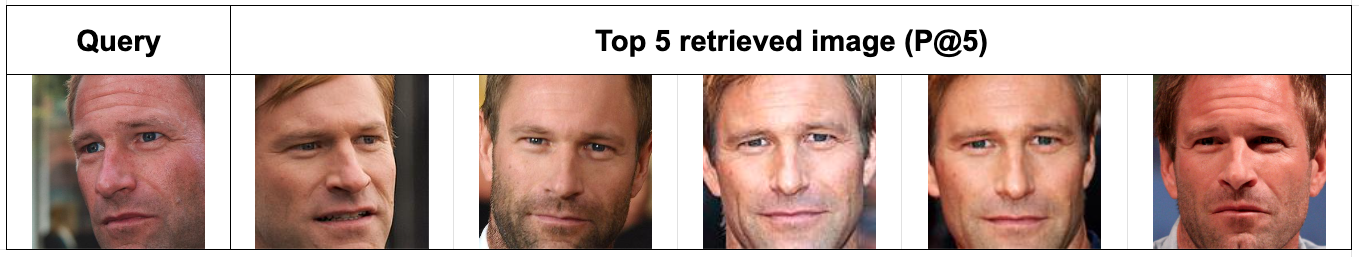
\includegraphics[width=0.8\textwidth]{images/face_retrieval_types.png} 
    \caption{Các dạng truy xuất ảnh mặt người}
    \label{fig:face_retrieval_types}
\end{figure}

\begin{itemize}
    \item[\textbf{Dạng: Truy xuất theo độ tương đồng }]
        \begin{itemize}
            \item[\textbf{Đầu vào:}] Ảnh khuôn mặt truy vấn.
            \item[\textbf{Đầu ra:}] Tập hợp \( K \) hình ảnh có độ tương đồng đặc trưng cao nhất so với ảnh truy vấn, không ràng buộc về danh tính.
        \end{itemize}
\end{itemize}
Đầu vào của các dạng trên đều là ảnh khuôn mặt truy vấn, riêng truy xuất theo đặc trưng cần kèm thêm điều kiện đặc trưng phụ. Đầu ra của dạng thứ nhất: tập hợp K hình ảnh trong cơ sở dữ liệu thuộc cùng danh tính, mức độ giống cao nhất với hình ảnh truy vấn. Đầu ra của dạng thứ hai: tập K hình ảnh có độ tương đồng đặc trưng cao nhất sao với hình ảnh truy vấn, không ràng buộc về danh tính. Đầu ra của dạng thứ ba trả về K hình ảnh vừa có độ tương đồng cao, vừa thoả mãn các đặc trưng phụ đã cho.


\section{Thách thức bài toán}
Việc xây dựng một mô hình truy xuất ảnh mặt người vừa gọn nhẹ vừa có khả năng mở rộng trên tập dữ liệu quy mô lớn phải đối mặt với nhiều thách thức đáng kể. Các thách thức này có thể được phân loại thành ba nhóm chính: thách thức liên quan đến dữ liệu, kiến trúc mô hình xác hiệu suất hệ thống. 

Thứ nhất, về mặt dữ liệu, các hệ thống phải xử lý sự biến đổi phức tạp vốn có trong ảnh mặt người. Một mặt, sự biến đổi trong cùng một danh tính (biến đổi nội lớp) là rất lớn, khi hình ảnh của cùng một các nhân có thể khác biệt đáng kể do sự thay đổi về góc chụp, điều kiện ánh sáng, biểu cảm, quá trình lão hoá, hay sự che khuất bởi các vật thể như khẩu trang, kính râm. Mặt khác, độ tương đồng giữa các biến đổi nội lớp lại có thể rất thấp, khi những cá nhân khác biệt lại sở hữu các đặc điểm khuôn mặt tương tự. Tình trạng này đòi hỏi mô hình phải có khả năng học được một không gian đặc trưng vừa đủ mạnh mẽ để khái quát hoá các biến thể trong cùng một lớp, vừa đủ sức phân biệt để tách bạch các lớp khác nhau. Thêm vào đó, quy mô dữ liệu khổng lồ với hàng triệu đến hàng tỷ hình ảnh làm gia tăng cấp số nhân chi phí tính toán và lưu trữ, đặt ra yêu cầu cấp thiết về hiệu quả trong cả quá trình huấn luyện và truy xuất.

Thứ hai, về kiến trúc mô hình, thách thức cốt lõi nằm ở sự đánh đổi giữa độ chính xác và hiệu quả tính toán. Các mô hình học sâu hiện đại có dung lượng lớn thường đạt độ chính xác cao nhờ khả năng biểu diễn mạnh mẽ, nhưng lại đòi hỏi tài nguyên tính toán khổng lồ, không phù hợp cho việc triển khai trên các thiết bị tài nguyên hạn chế. Do đó, việc thiết kế một kiến trúc mạng gọn nhẹ nhưng vẫn duy trì được khả năng trích xuất đặc trưng có sức phân biệt cao là một bài toán khó. Điều này gắn liền với thách thức về việc học một biểu diễn đặc trưng cô đặc. Việc giảm số chiều của vector đặc trưng là tối quan trọng để tiết kiệm bộ nhớ và tăng tốc độ tìm kiếm, nhưng quá trình này có nguy cơ làm mất mát thông tin nhận dạng quan trọng.

Cuối cùng, về hiệu suất hệ thống, mô hình phải đáp ứng được yêu cầu về tốc độ truy xuất trong thời gian thực. Với có sở dữ liệu quy mô lớn, việc tìm kiếm tuần tự qua toàn bộ dữ liệu là bất khả thi về mặt thời gian. Điều này đòi hỏi phải tích hợp các thuật toán lập chỉ mục và tìm kiếm lân cận gần đúng hiệu quả. Hơn nữa, mục tiêu cuối cùng là triển khai trên các thiết bị biên như điện thoại di động hay camera thông minh, vốn bị giới hạn nghiêm ngặt về năng lực xử lý, bộ nhớ và năng lượng. Do đó, toàn bộ hệ thống, từ mô hình trích xuất đặc trưng đến thuật toán tìm kiếm, phải được tối ưu hoá để hoạt động hiệu quả trong một môi trường tài nguyện bị ràng buột chặt chẽ.
\section{Giới hạn bài toán}
\section{Hướng tiếp cận}
\section{Đóng góp}
\section{Tổ chức khóa luận}
\section{Tổng kết}

\newpage


%Tóm tắt luận văn được trình bày nhiều nhất trong 24 trang in trên hai mặt giấy, cỡ chữ Times New Roman 11 của hệ soạn thảo Winword hoặc phần mềm soạn thảo Latex đối với các chuyên ngành thuộc ngành Toán.

%Mật độ chữ bình thường, không được nén hoặc kéo dãn khoảng cách giữa các chữ.
%Chế độ dãn dòng là Exactly 17pt.
%Lề trên, lề dưới, lề trái, lề phải đều là 1.5 cm.
%Các bảng biểu trình bày theo chiều ngang khổ giấy thì đầu bảng là lề trái của trang.
%Tóm tắt luận án phải phản ảnh trung thực kết cấu, bố cục và nội dung của luận án, phải ghi đầy đủ toàn văn kết luận của luận án.
%Mẫu trình bày trang bìa của tóm tắt luận văn (phụ lục 1).

\chapter{Trình bày báo cáo}
\label{Chapter2}

\section{Quy định chung}

Báo cáo phải được trình bày ngắn gọn, rõ ràng, mạch lạc, sạch sẽ, không được tẩy xóa, có đánh số trang, đánh số bảng biểu, hình vẽ, đồ thị. 

Nội dung báo cáo được phân thành các chương. Số thứ tự của các chương, mục được đánh số bằng hệ thống số Ả-rập, không dùng số La mã. Các mục và tiểu mục được đánh số bằng các nhóm hai hoặc ba chữ số, cách nhau một dấu chấm: số thứ nhất chỉ số chương, chỉ số thứ hai chỉ số mục, số thứ ba chỉ số tiểu mục.


%Báo cáo cần dùng LaTEX để viết và trình bày theo mẫu đã được cung cấp.

 Báo cáo trình bày sử dụng khổ giấy A4 với việc canh lề như sau: Lề trên 3 cm, lề dưới 2,5 cm, lề trái 3 cm, lề phải 2 cm. Đánh số trang ở giữa bên dưới. Các trang trước phần nội dung (Lời cảm ơn, Mục lục, \ldots), các trang được đánh số sử dụng chữ số la mã viết thường (i, ii, iii,\ldots). Các trang nằm trong phần nội dung (Chương 0 hoặc Chương 1,\ldots) thì số trang được đánh theo chữ số Ả-rập (1, 2, 3,\ldots).

Font chữ dùng trong báo cáo (Times New Roman) với kích cỡ (size) 13-14pt, sử dụng chế độ dãn dòng (line spacing) 1,5 lines.

%Các bảng biểu trình bày theo chiều ngang khổ giấy thì đầu bảng là lề trái của trang. 


\section{Bố cục của báo cáo}

Nội dung của báo cáo tối thiểu 50 trang khổ A4 và không nên vượt quá 100 trang (không kể các trang bìa, lời cám ơn, mục lục, tài liệu tham khảo, phụ lục, \ldots) theo trình tự như sau:

\begin{itemize}
\item MỞ ĐẦU (thường đặt tên là ``Giới thiệu''): Trình bày lý do chọn đề tài, mục đích, đối tượng và phạm vi nghiên cứu.
Mô tả bài toán mà đề tài giải quyết.
Bài toán này có gì hay?
Tại sao lại cần giải quyết bài toán này?
Bài toán này có gì khó?
Có những hướng nào để giải quyết bài toán này?
Những hướng giải quyết trước đây có những vấn đề gì chưa giải quyết được?
Các câu hỏi nghiên cứu mà đề tài trả lời hoặc những vấn đề mà đề tài sẽ giải quyết.
Các đóng góp của đề tài.

\item TỔNG QUAN (thường đặt tên là ``Các công trình liên quan''): Phân tích đánh giá các hướng nghiên cứu đã có của các tác giả trong và ngoài nước liên quan đến đề tài; nêu những vấn đề còn tồn tại (những vấn đề nào mà các công trình khác chưa giải quyết được); chỉ ra những vấn đề mà đề tài cần tập trung, nghiên cứu giải quyết.

\item NGHIÊN CỨU THỰC NGHIỆM HOẶC LÝ THUYẾT (thường đặt tên là ``Phương pháp đề xuất''): Trình bày cơ sở lý thuyết, lý luận, giả thiết khoa học và phương pháp nghiên cứu đã được sử dụng trong đề tài.

Nếu đề xuất hướng giải quyết mới, mô hình mới thì cần mô tả chi tiết cách giải quyết của mình (chi tiết tới mức người khác có thể dựa vào phần này mà cài đặt lại được đúng hoàn toàn phương pháp của mình đề ra).

\item TRÌNH BÀY, ĐÁNH GIÁ BÀN LUẬN VỀ CÁC KẾT QUẢ (thường đặt tên là ``Kết quả thí nghiệm''): Mô tả các kết quả nghiên cứu khoa học hoặc kết quả thực nghiệm.
Đối với  đề tài ứng dụng có kết quả là sản phẩm phần mềm phải có hồ sơ thiết kế, cài đặt,\ldots theo một trong các mô hình đã học (UML,\ldots).

Thông thường cần mô tả môi trường thí nghiệm trước như sử dụng dữ liệu nào, dùng độ đo nào để đánh giá, môi trường chạy thí nghiệm (cấu hình máy nếu cần phân tích thông tin về thời gian chạy thực nghiệm). Sau đó, nêu kết quả thực nghiệm, bàn luận và giải thích kết quả.

\item KẾT LUẬN VÀ HƯỚNG PHÁT TRIỂN (thường đặt tên là ``Kết luận''): Trình bày những kết quả đạt được, những đóng góp mới và những đề xuất mới, kiến nghị về những hướng nghiên cứu tiếp theo.

\item DANH MỤC TÀI LIỆU THAM KHẢO: Chỉ bao gồm các tài liệu được trích dẫn, sử dụng và đề cập tới để bàn luận trong báo cáo.
Phần này các bạn chuẩn bị 1 file BIB để lưu các tài liệu trích dẫn.
Khi các bạn trích dẫn một tài liệu nào đó, LaTeX sẽ tự động thêm vào danh mục tài liệu tham khảo giúp các bạn.
Các bạn xem hướng dẫn cách trích dẫn ở chương sau.

\item PHỤ LỤC: Phần này bao gồm nội dung cần thiết nhằm minh họa hoặc hỗ trợ cho nội dung báo cáo như số liệu, mẫu biểu, tranh ảnh,\ldots Phụ lục không được dày hơn phần chính của báo cáo.
Nếu có công trình công bố thì để vào phần phụ lục này.
\end{itemize}

\section{Bảng biểu, hình vẽ, phương trình}

%Những qui định dưới này các bạn có thể bỏ qua hoặc đọc để hiểu thêm.
%Những định dạng này LaTeX đều tự động giúp các bạn.
%Các bạn xem hướng dẫn chi tiết hơn ở chương sau.

Việc đánh số bảng biểu, hình vẽ, phương trình phải gắn với số chương; ví dụ hình 3.4 có nghĩa là hình thứ 4 trong Chương 3.
Mọi đồ thị, bảng biểu, hình vẽ lấy từ các nguồn khác phải được trích dẫn đầy đủ.

\subsection{Bảng biểu, hình vẽ}



Đầu đề của bảng biểu ghi phía trên bảng, đầu đề của hình vẽ ghi phía dưới hình.

Thông thường, những bảng ngắn và đồ thị phải đi liền với phần nội dung đề cập tới các bảng và đồ thị này ở lần thứ nhất.
Các bảng dài có thể để ở những trang riêng nhưng cũng phải tiếp theo ngay phần nội dung đề cập tới bảng này ở lần đầu tiên.
Các bảng rộng vẫn nên trình bày theo chiều đứng dài 297mm của trang giấy, chiều rộng của trang giấy có thể hơn 210mm.
Chú ý gấp trang giấy sao cho số và đầu đề của hình vẽ hoặc bảng vẫn có thể nhìn thấy ngay mà không cần mở rộng tờ giấy.
Tuy nhiên hạn chế sử dụng các bảng quá rộng này.

Đối với những trang giấy có chiều đứng hơn 297mm (bản đồ, bản vẽ,\ldots) thì có thể để trong một phong bì cứng đính bên trong bìa sau của báo cáo.

Các hình vẽ phải sạch sẽ bằng mực đen để có thể sao chụp lại; có đánh số và ghi đầy đủ đầu đề, cỡ chữ phải bằng cỡ chữ sử dụng trong báo cáo.

Khi đề cập đến các bảng biểu và hình vẽ phải nêu rõ số của hình và bảng biểu đó, ví dụ ``... được nêu trong Bảng 4.1'' hoặc ``xem Hình 3.2'' mà không được viết ``… được nêu trong bảng dưới đây'' hoặc ``trong đồ thị của X và Y sau''.

\subsection{Phương trình toán học}

Việc trình bày phương trình toán học trên một dòng đơn hoặc dòng kép tùy ý, tuy nhiên phải thống nhất trong toàn báo cáo.

Khi ký hiệu xuất hiện lần đầu tiên thì phải giải thích và đơn vị tính phải đi kèm ngay trong phương trình có ký hiệu đó.
Nếu cần thiết, danh mục của tất cả các ký hiệu, chữ viết tắt và nghĩa của chúng cần được liệt kê và để ở phần đầu của báo cáo.

Tất cả các phương trình cần được đánh số và để trong ngoặc đơn đặt bên phía lề phải.
Nếu một nhóm phương trình mang cùng một số thì những số này cũng được để trong ngoặc, hoặc mỗi phương trình trong nhóm phương trình (5.1) có thể được đánh số là (5.1.1), (5.1.2), (5.1.3).

\section{Viết tắt}

\textbf{Không lạm dụng việc viết tắt} trong báo cáo.
Chỉ viết tắt những từ, cụm từ hoặc thuật ngữ được sử dụng nhiều lần trong báo cáo.
Không viết tắt những cụm từ  dài, những mệnh đề; không viết tắt những cụm từ ít xuất hiện trong báo cáo.
Nếu cần viết tắt những từ thuật ngữ, tên các cơ quan, tổ chức,\ldots thì được viết tắt sau lần viết thứ nhất có kèm theo chữ viết tắt trong ngoặc đơn.
Nếu báo cáo có nhiều chữ viết tắt thì phải có bảng danh mục các chữ viết tắt (xếp theo thứ tự ABC) ở phần đầu báo cáo.

Nhắc lại: \textbf{không lạm dụng việc viết tắt} trong báo cáo.
Khi các bạn sử dụng từ viết tắt, người đọc sẽ phải lật lại những phần đã đọc, để tìm lại xem từ viết tắt đó nghĩa là gì.
Việc này sẽ làm chậm tốc độ đọc và sẽ khiến người đọc khó theo dõi báo cáo của bạn hơn.
Nếu có thể, hạn chế hoàn toàn việc dùng viết tắt.

\section{Tài liệu tham khảo và cách trích dẫn}

Mọi ý kiến, khái niệm có ý nghĩa, mang tính chất gợi ý không phải của riêng tác giả và mọi tham khảo khác phải được trích dẫn và chỉ ra nguồn trong danh mục Tài liệu tham khảo của báo cáo. Nguồn được trích dẫn phải được liệt kê chính xác trong danh mục Tài liệu tham khảo.

Việc trích dẫn, tham khảo chủ yếu nhằm thừa nhận nguồn của những ý tưởng có giá trị giúp người đọc theo được mạch suy nghĩ của tác giả, không làm trở ngại việc đọc.


Không trích dẫn những kiến thức phổ biến, mọi người đều biết cũng như không làm báo cáo nặng nề với những tham khảo trích dẫn.

Nếu không có điều kiện tiếp cận được một tài liệu gốc mà phải trích dẫn thông qua một tài liệu khác thì phải nêu ra trích dẫn này, đồng thời tài liệu gốc đó không được liệt kê trong danh mục tài liệu tham khảo của báo cáo.

%\chapter{Hướng dẫn sử dụng template}
\chapter{Phương pháp}
\label{Chapter3}

\section{Mạng lượng tử hoá tích trực chuẩn cho truy xuất ảnh khuôn mặt quy mô lớn}
\subsection{Tổng quan về mạng lượng tử hoá tích trực chuẩn}
Mạng lượng tử hoá tích trực chuẩn là một mạng nơ-ron sử dụng lượng tử hoá với ràng buộc vuông góc, sử dụng bộ mã được định nghĩa trước nhằm tăng độ phân biệt và giảm sự dư thừa giữa các thông tin đặc trưng với nhau, giải quyết các thách thức về biến đổi nội lớp như tư thế, ánh sáng, biểu cảm. Khả năng tổng quá hoá cao, phù hợp với nhu cầu truy xuất các danh tính chưa từng thấy.

\begin{figure}[htbp] % hoặc [htbp]
    \centering
    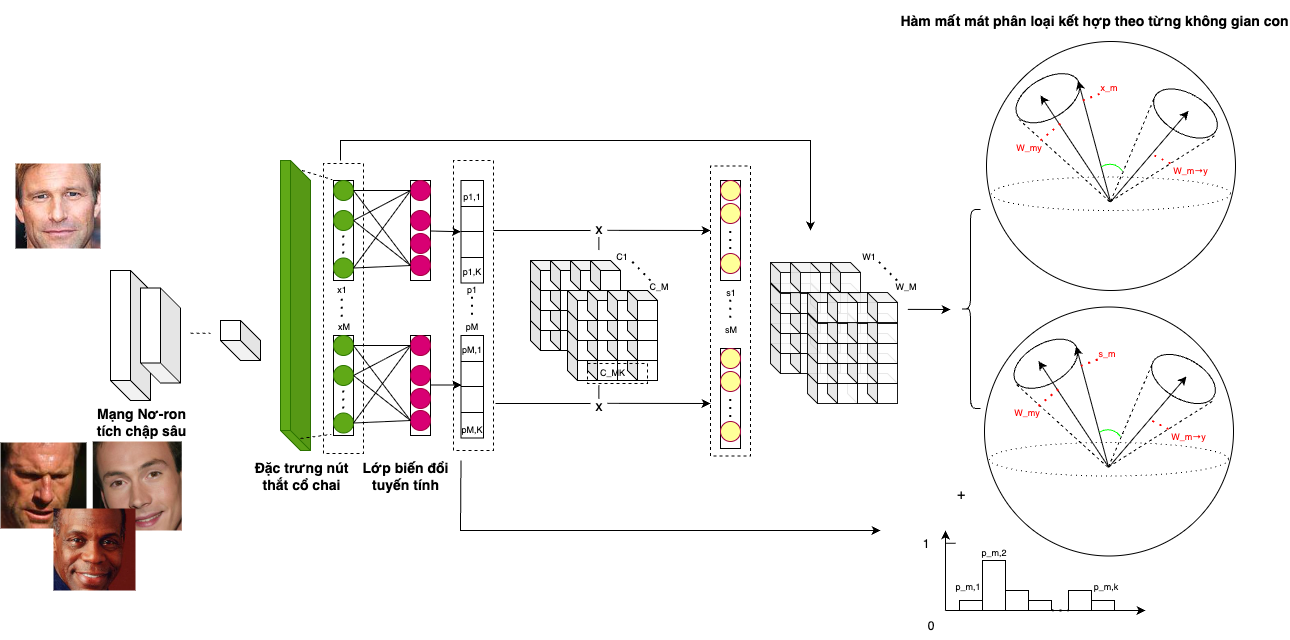
\includegraphics[width=0.8\textwidth]{images/opqn_model.png} 
    \caption{Mô hình lượng tử hoá tích trực chuẩn}
    \label{fig:opqn_rmodel_types}
\end{figure}

Các thành phần chính và kiến trúc của mạng lượng tử hoá tích trực chuẩn bao gồm các thành phần cốt lõi như sau: Mạng xương sống, lượng tử hoá mềm thông qua khử tương quan đặc trưng - xác suất, sinh mã từ trực chuẩn, hàm mất mát phân loại kết hợp theo từng không gian con, tối thiểu hoá độ cô đặc cho việc gán mã one-hot, quá trình học và tối ưu hoá và khoảng cách bất đối xứng trong truy xuất.
\subsection{Các ký hiệu và ký pháp}
Trong mô hình OPQN, các ký hiệu và ký pháp được định nghĩa để mô tả rõ ràng các thành phần dữ liệu, đặc trưng, và hàm mất mát. Bảng \ref{tab:terms_part1} và \ref{tab:terms_part2} trình bày chi tiết các ký hiệu này, được sử dụng xuyên suốt phần phương pháp để giải thích quy trình lượng tử hóa và tối ưu hóa.

\begin{table}[h!]
    \centering
    \begin{tabular}{|c|p{3cm}|p{6cm}|}
        \hline
        \textbf{Ký hiệu} & \textbf{Ký pháp} & \textbf{Mô tả} \\ \hline
        $I_i$ & $\{I_i\}_{i=1}^N$ & Tập hợp $N$ hình ảnh khuôn mặt đầu vào. \\ \hline
        $y_i$ & $y \in \mathbb{R}^N$ & Nhãn danh tính tương ứng với hình ảnh $I_i$. \\ \hline
        $x_i$ & $x_i = f(\Theta, I_i) \in \mathbb{R}^D$ & Đặc trưng nút cổ chai được trích xuất từ hình ảnh $I_i$ bởi mạng xương sống với tham số $\Theta$, có chiều $D$. \\ \hline
        $x_{im}$ & $x_{im} \in \mathbb{R}^d$ & Vector con thứ $m$ của ảnh đặc trưng $x_i$, với $d = D/M$ và $m = 1, \dots, M$. \\ \hline
        $M$ & $M$ & Số lượng vectơ con mà đặc trưng $x_i$ được chia thành. \\ \hline
        $d$ & $d = D/M$ & Chiều của mỗi vector con $x_{im}$. \\ \hline
        $C$ & $C = [C_1, \dots, C_M]$ & Tập hợp $M$ bộ mã, mỗi bộ mã $C_m \in \mathbb{R}^{d \times K}$ chứa $K$ từ mã trực chuẩn. \\ \hline
        $C_{mk}$ & $C_{mk} \in \mathbb{R}^d$ & Từ mã thứ $k$ trong bộ mã $C_m$. \\ \hline
        $F$ & $F = [F_1, \dots, F_M]$ & Tập hợp ma trận tham số của các lớp tuyến tính, với $F_m \in \mathbb{R}^{d \times K}$. \\ \hline
        $F_{mk}$ & $F_{mk} \in \mathbb{R}^d$ & Vectơ tham số thứ $k$ trong ma trận $F_m$. \\ \hline
        $p_{im}$ & $p_{im} = [p_{im,1}, \dots, p_{im,K}] \in \mathbb{R}^K$ & Vector xác suất của vector con $x_{im}$, được tính qua softmax: $p_{im,k} = \frac{e^{x_{im}^T F_{mk}}}{\sum_{j=1}^K e^{x_{im}^T F_{mj}}}$. \\ \hline
        $s_{im}$ & $s_{im} = \sum_{k=1}^K p_{im,k} \cdot C_{mk}$ & Lượng tử hóa mềm của vectơ con $x_{im}$. \\ \hline
        $h_{im}$ & $h_{im} = C_{m k^*}$, $k^* = \arg\max_k p_{im,k}$ & Lượng tử hóa cứng của vectơ con $x_{im}$. \\ \hline
    \end{tabular}
    \caption{Phần 1: Ký hiệu và ký pháp (Dữ liệu và đặc trưng)}
    \label{tab:terms_part1}
\end{table}

\begin{table}[h!]
    \centering
    \begin{tabular}{|c|p{6cm}|p{5cm}|}
        \hline
        \textbf{Ký hiệu} & \textbf{Ký pháp} & \textbf{Mô tả} \\ \hline
        $W$ & $W = [W_1, \dots, W_M]$ & Tập hợp trọng số của các bộ phân lớp theo không gian con, với $W_m \in \mathbb{R}^{d \times C}$. \\ \hline
        $W_{mc}$ & $W_{mc} \in \mathbb{R}^d$ & Trọng số của lớp $c$ trong bộ phân lớp $W_m$. \\ \hline
        $L_x$ & $L_x = \sum_{i=1}^N \sum_{m=1}^M -\log \frac{e^{r (\cos \theta_{y_i, x_{im}} - u)}}{e^{r (\cos \theta_{y_i, x_{im}} - u)} + \sum_{j \neq y_i} e^{r \cos \theta_{j, x_{im}}}}$ & Hàm mất mát phân lớp cho đặc trưng gốc $x_{im}$ dựa trên softmax với biên góc $u$ và tham số $r$. \\ \hline
        $L_s$ & Tương tự $L_x$ & Hàm mất mát phân lớp cho lượng tử hóa mềm $s_{im}$. \\ \hline
        $L_{clf}$ & $L_{clf} = \frac{1}{2MN} (L_x + L_s)$ & Hàm mất mát phân lớp liên hợp theo không gian con. \\ \hline
        $L_{ent}$ & $L_{ent} = -\frac{1}{MN} \sum_{i=1}^N \sum_{m=1}^M \sum_{k=1}^K p_{im,k} \log p_{im,k}$ & Hàm mất mát entropy để khuyến khích $p_{im}$ gần với one-hot. \\ \hline
        $L$ & $L = L_{clf} + \lambda L_{ent}$ & Hàm mất mát tổng, với $\lambda$ là trọng số điều chỉnh. \\ \hline
        $\Theta$ & $\Theta$ & Tham số của mạng xương sống. \\ \hline
        $A$ & $A_{ij} = \cos\left[j\pi \cdot \frac{i + \frac{1}{2}}{d}\right]$ & Ma trận cơ sở trực chuẩn được sinh bởi DCT-II cho các từ mã. \\ \hline
        $K$ & $K \leq d$ & Số lượng các từ mã trong mỗi bộ mã $C_m$. \\ \hline
        $u$ & $u$ & Biên góc trong hàm mất mát phân lớp. \\ \hline
        $r$ & $r$ & Tham số điều chỉnh trong hàm mất mát phân lớp. \\ \hline
    \end{tabular}
    \caption{Phần 2: Ký hiệu và ký pháp (Hàm mất mát và tham số)}
    \label{tab:terms_part2}
\end{table}


Các ký hiệu này sẽ được áp dụng trong các phân đoạn sau để mô tả chi tiết quy trình lượng tử hóa mềm, sinh từ mã trực chuẩn, huấn luyện và truy xuất mô hình OPQN.

\subsection{Lượng tử hoá mềm thông qua khử tương quan đặc trưng - xác suất}

\subsubsection{Lượng tử hoá mềm và Lượng tử hoá cứng}
Lượng tử hoá trong học máy và thị giác máy tính là quá trình ánh xạ một vectơ đặc trưng liên tục về một tập hữu hạn các từ mã trong bộ mã. Lượng tử hoá được chia thành hai loại: Lượng tử hoá cứng và lượng tử hoá mềm. Trong đó, lượng tử hoá cứng ánh xạ đặc trưng vào một từ mã duy nhất ở gần nhất, lượng tử hoá mềm ánh xạ mỗi  đặc trưng vào tổ hợp tuyến tính của nhiều từ mã, với trọng số là xác suất.

Mặc dù lượng tử hoá cứng có độ phức tạp tính toán nhanh hơn so với lượng tử hoá mềm, nhưng lại không khả vi vì hàm chọn từ mã gây gián đoạn tính toán độ dốc, ảnh hưởng đến quá trình lan truyền ngược. Thêm vào đó, độ mất mát thông tin của lượng tử hoá cứng cao, mỗi vectơ chỉ ánh xạ đến một từ mã gần nhất. Vì thế cho nên, nghiên cứu không dùng lượng tử hoá cứng trong việc lượng tử hoá ảnh đầu vào để huấn luyện mô hình. Thay vào đó, tận dụng tốc độ tính toán nhanh của chúng cho việc lượng tử hoá hàng triệu ảnh lưu cơ sở dữ liệu, phục vụ quá trình truy xuất thông tin diễn ra với tốc độc cao và giảm chi phí tính toán.

Ngược lại, lượng tử hoá mềm phục vụ mô hình trong việc huấn luyện đầu-cuối nhờ tính khả vi của hàm trung bình mũ, độ dốc được giữ liên tụ. Độ mất mát thông tin thấp hơn do lượng tử hoá mềm là một tổ hợp tuyến tính có trọng số là xác xuất trên tập hữu hạn các từ mã, tránh mất mát các thông tin đặc trưng quan trọng, đặc biệt là các đặc trưng của biến thể nội lớp.

% Khử tương quan đặc trưng-xác suất vs Các phương pháp lượng tử hoá truyền thống 
Bên cạnh sự phân loại trên, nghiên cứu không chỉ dừng ở việc so sánh giữa lượng tử hoá cứng và mềm, mà còn tập trung vào khử tương quan đặc trưng và sử dụng xác suất trong ánh xạ, thay thế các phương pháp lượng tử hoá truyền thống.

\subsubsection{Vấn đề của lượng tử hoá tích} 
Trong lượng tử hoá tích (PQ) truyền thống, vectơ đặc trưng $x \in \mathbb{R}^D$ được chia thành nhiều vectơ con $x = [x_1, x_2,...,x_M]$, $x \in \mathbb{R}^{D/M}$, $x_{i,m} = [x_{i,1}, x_{i,2},...,x_{1,d}]$. Tuy nhiên, có ba hạn chế mà phép lượng tử hoá tích gặp phải: Tương quan đặc trưng chưa được xử lý, lượng tử hoá gây mất mát thông tin ngữ nghĩa, độ chính xác của truy xuất giảm đối do sai số lượng tử hoá. 

Thứ nhất, trong nhiều đặc trưng từ CNN, các chiều thường tương quan mạnh, thông tin về một yếu tố như ánh sáng, kiểu dáng, etc.. có thể trải trên nhiều chiều, nhưng việc chia vectơ đặc trưng $x$ thành nhiều vectơ con $x_m$ và lượng tự hoá độc lập chúng với từng từ mã $C_m$, điều này ngầm giả định rằng các vectơ con là tương đối độc lập. Khi biểu diễn tương quan qua ma trận hiệp phương sai $\Sigma = \mathbb{E}[(x-\mu)(x-\mu)^T]$, nếu $\Sigma$ có nhiều phần tử ngoài đường chéo lớn, nghĩa là các chiều phụ thuộc nhau, khi chia theo chỉ số, các không gian con thường không trùng với các trục chính của phân phối, tức là các thành phần có phương sai lớn và phụ thuộc lẫn nhau có thể nằm dàn trải qua nhiều không gian con. Hệ quả rằng các bộ mã độc lập cho từng không gian con không thể mô tả tốt các mối liên hệ chéo giữa các chiều, làm sai số lượng tử lớn hơn so với việc lượng tử hoá chung -tối ưu hoá toàn cục, bên cạnh đó sai số khôi phục tăng, làm giảm chất lượng truy hồi, đặc biệt với dữ liệu có cấu trúc ngữ nghĩa mạnh. 

Thứ hai, mất mát thông tin khi chia các vectơ con, nếu có một thông tin ngữ nghĩa nào đó phụ thuộc vào sự phối hợp của nhiều chiều nằm ở các vectơ con khác nhau, thì khi cắt ra và lượng tử hoá độc lập chúng, ta sẽ phá vỡ mối quan hệ đó, gây mất mát thông tin ngữ nghĩa. Hệ quả của việc chia vectơ đặc trưng thành các vectơ con và lượng tử hoá chúng theo phương pháp lượng tử hoá tích, các khác biệt tinh tế giữa các mẫu ảnh sẽ bị làm mờ, và các bộ mã dù có tổ hợp các trung tâm mã trong bộ mã lớn, nhưng không thể biểu diễn chính xác quan hệ chéo.

Thứ ba, độ chính xác truy hồi giảm do sai số lượng tử hoá, trong phương pháp tiìm kiếm láng giềng gần nhất, ta quan tâm đến xếp hạng khoảng cách giữa truy vấn $q$ và các vectơ dữ liệu $x$. Với lượng tử hoá tích, ta đo khoảng cách $\|q - x\|^2 \;\approx\; \sum_{m=1}^M \|q_m - c_{m,k_m}\|^2$, nhưng nếu $\hat{x}$ ($x$ sau khi lượng tử hoá) khác xa $x$ do sai số lượng tử hoá lớn, thì khoảng cách tính bị sai lệch, dẫn đến thứ tự xếp hạng truy xuất thay đổi.

\subsubsection{Khử tương quan đặc trưng-xác suất}
Để khắc phục các hạn chế nêu trên của phương pháp lượng tử hoá tích, bài báo OPQN đề xuất cơ chế khử tương quan đặc trưng - xác suất.

Thay vì ánh xạ trực tiếp vectơ con vào các từ mã bằng khoảng cách Ơ-clid như trong lượng tử hoá tích, OPQN chèn thêm một tầng tuyến tính. Với mỗi vectơ con $x_{im}$, tầng này chiếu đặc trưng sang một không gian mới, rồi tính điểm tương ứng cho từng từ mã. Sau đó, các điểm này đi qua hàm trung bình mũ để tạo thành phân phối xác suất gán cho các từ mã. Cốt lõi của cơ chế khử tương quan nằm ở chỗ đặc trưng không còn gắn trực tiếp với các vectơ con độc lập, mà được ánh xạ sang một không gian xác suất. Công thức được tính như sau:


\begin{equation}
p_{im,k} = \frac{\exp\!\left(x_{im}^{T} F_{m,k}\right)}
{\sum_{j=1}^{K} \exp\!\left(x_{im}^{T} F_{m,j}\right)}
\end{equation}


\begin{itemize}
    \item \textbf{Đầu vào:} $x_{im}$ vectơ đặc trưng con thứ $m$ của ảnh $i$.
    \item \textbf{Tham số học được:} $F_{m,k}$ ma trận tham số của tầng tuyến tính.
    \item \textbf{Đầu ra:} $p_{im,k}$ xác suất vectơ thuộc về từ mã thứ $k$.
\end{itemize}

Nhờ lớp trung gian $F_{m,k}$, quá trình mã hoá không còn dựa duy nhất vào khoảng cách hình học như trong phân cụm truyền thống, mà trở thành \textbf{một phép học xác suất mềm} giữa đặc trưng và các từ mã, xác xuất $p_{im,k}$ được điều chỉnh để tối ưu mục tiêu của toàn bộ mô hình. Thay vì gán vào một từ mã cứng nhắc, mô hình học ma trận tham số $F_{m,k}$ qua quá trình huấn luyện mạng nơ-ron. Cơ chế này cho phép mô hình linh hoạt hơn, tận dụng thông tin từ nhiều từ mã và được tối ưu cùng với toàn bộ mạng.

Thứ hai, OPQN sử dụng các từ mã trực chuẩn (chi tiết ở mục 3.1.4), làm giảm tương quan ngầm giữa các đặc trưng và bộ mã, giúp phân phối xác suất có ý nghĩa rõ ràng.

\subsubsection{Xây dựng lượng tử hoá mềm}
Sau khi xác định vectơ xác suất $p_{im,k}$ qua hàm softmax, lượng tử hoá mềm $s_{im}$ được xây dựng bằng cách kết hợp tuyến tính các từ mã $C_{mk}$ với các giá trị xác suất tương ứng. Công thức được biểu diễn như sau:

\begin{equation}
s_{im} = \sum_{k=1}^K p_{im,k} . C_{mk}
\end{equation}

Trong đó, $C_{mk}$ là từ mã thứ $k$ trong bộ mã $C_m$ của không gian con thứ m, và $p_{im,k}$ là xác xuất gán được tính từ $x_{im}$ và tham số $F_{mk}$. Kết quả $s_{im}$ là một tổ hợp lồi của các từ mã, với tổng các xác suất $p_{im,k}$ bằng một, và giá trị không âm. Điều này cho phép $s_{im}$ tái hiện vectơ con $x_{im}$ một cách mềm mại, giảm thiểu lỗi lượng tử hoá so với việc gán cứng vào một từ mã duy nhất.

Một đặc điểm quan trọng trong OPQN là việc tách biệt quá trình gán xác suất $p_{im,k}$ với các từ mã $C_{mk}$, giúp giảm sự phụ thuộc vào dữ liệu huấn luyện. Sự độc lập này cho phép $p_{im,k}$ được học một cách linh hoạt, trong khi các từ mã giữ vai trò cố định, góp phần tăng khả năng tổng quát hoá trên các tập dữ liệu mới, đặc biệt với các biến thể khuôn mặt chưa thấy. Ngoài ra, cách tiếp cận này tránh được những  những hạn chế của PQ, như hiện tượng bộ mã bị ảnh hưởng bởi độ chệch dữ liệu, đảm bảo độ ổn định và hiệu quả trong tìm kiếm quy mô lớn. Nhờ vậy, $ s_{im} $ không chỉ cải thiện độ chính xác mà còn hỗ trợ tính toán khoảng cách bất đối xứng trong giai đoạn tìm kiếm sau này.

\subsubsection{Xây dựng lượng tử hoá cứng}
Sau khi xây lượng tử hoá mềm $s_{im}$, OPQn chuyển sang phương pháp lượng tử hoá cứng trong giai đoạn kiểm tra để tối ưu hoá hiệu suất tìm kiếm. Quá trình này được thực hiện bằng cách xác định chỉ số $k^*$ của từ mã có xác suất cao nhất trong vectơ xác suất $p_{im}$. Công thức được biểu diễn như sau:

\begin{equation}
k^* = \arg _{k = 1,2,...,K}\max p_{im,k}
\end{equation}

Trong đó, giá trị $k^*$ là chỉ số của từ mã trong bộ mã $C_m$, mà có khả năng tái hiện tốt nhất vector $x_{im}$, tức là giá trị có xác suất gán lớn nhất trên phân phối xác suất $p_{im}$. Từ $k*$, lượng tử hoá cứng $h_{im}$ được định nghĩa đơn giản là:

\begin{equation}
h_{im} = C_{mk^*}
\end{equation}

Ở đây, $C_{mk^*}$ là từ mã tương ứng với từ mã thứ $k*$ trong bộ mã $C_m$. Phương pháp này chuyển đổi biểu diễn mềm $x_{im}$ thành một vector rời rạc $h_{im}$, phù hợp cho việc tính toán nhanh khoảng cách trong hệ thống truy xuất thông tin với quy mô lớn. Khác với giai đoạn huấn luyện, nơi lượng tử hoá mềm được ưu tiên để tối ưu hoá độ dốc, lượng tử hoá cứng chỉ được áp dụng trong giai đoạn truy xuất, để giảm độ phức tạp tính toán và bộ nhớ, đặc biệt khi sửa dụng bảng tra cứu để so sánh khoảng cách bất đối xứng. 

Việc sử dụng $k^*$ đảm bảo rằng mỗi vector con $x_{im}$ được ánh xạ chính xác vào một từ mã đại diện, giúp duy trì tính phân biệt của đặc trưng trong khi tối ưu hoá hiệu suất. Điều này quan trọng trong ứng dụng truy xuất khuôn mặt, nơi độ chính xác của phép gán từ mã ảnh hưởng trực tiếp đến kết quả hàng xóm gần nhất. Phương pháp này tận dụng lợi thế của quá trình học trước đó ($p_{im,k}$ và $s_{im}$) để đạt được sự cân bằng giữa độ chính xác và tốc độ, đặt nền móng cho các bước tìm kiếm hiệu quả trong OPQN.

\subsection{Sinh từ mã trực chuẩn}
\subsubsection{Vấn đề của bộ mã trong phương pháp lượng tử hoá truyền thống và hướng khắc phục} 
Trong các phương pháp lượng tử hoá tích truyền thống, bộ mã thường được học trực tiếp từ dữ liệu thông qua thuật toán như phân cụm K-Means. Cách tiếp cận này dẫn đến sự phụ thuộc mạnh mẽ của bộ mã vào phân bố của tập dữ liệu, có thể gây ra hiện tượng dư thừa thông tin giữa các từ mã hoặc lệch lạc từ mã khi dữ liệu không đại diện đầy đủ cho không gian đặc trưng. Giả định có một tập huấn luyện với độ chệch về một số loại hình ảnh, như tư thế hoặc ánh sáng nhất định, khả năng tổng quá hoá sẽ giảm khi áp dụng mô hình này trên dữ liệu mới hoặc danh tính chưa thấy, do bộ mã có thể bị học lệch.

Để khắc phục những hạn chế này, OPQN sử dụng các từ mã cố định và trực chuẩn, không phụ thuộc vào dữ liệu huấn luyện vì đã được thiết kế trước. Cách tiếp cận này đảm bảo tính ổn định và tính toán hiệu quả, đồng thời tăng cường chất lượng lượng tử hoá bằng cách tận dụng các đặc tính toán học cố định. 

Bằng cách này, OPQN chuyển thách thức từ việc học các từ mã sang việc học gán xác suất (như đã trình bày ở phần 3.1.3), giúp mô hình tăng khả năng khái quát hoá và giảm rủi ro với dữ liệu có tính biến thiên cao.

% Tính chất của từ mã trực chuẩn
Các từ mã trực chuẩn trong OPQN là các vector trong bộ mã $C_m$ thoả mãn hai điều kiện chính: Trực giao lẫn nhau và chuẩn hoá về độ dài bằng một. Cụ thể, đối với bất kỳ hai từ mã $C_{mk}$ và $C_{mj}$ ($k \neq j$ trong cùng một bộ mã $C_m \in \mathbb{R}^{d \times K}$, ta có:

$C^T_{mk} C_{mj} = 0$ (trực giao), $\|C_{mk}\| = 1$ (chuẩn hoá)

Hai đặc tính của từ mã trực chuẩn mạng lại các lợi ích quan trọng như sau:

Thứ nhất, các từ mã không dư thừa và phân bố đồng đều trong không gian $\mathbb{R}^d$, phép trực giao đảm bảo tính không chồng chéo thông tin, tránh các dư thừa thường gặp đối với các bộ mã học từ dữ liệu. Thêm vào đó, đặc tính này giúp bao phủ toàn bộ không gian vector con một cách hiệu quả, tăng khả năng biểu diễn đa dạng các đặc trưng khuôn mặt và những biến thể nội lớp.

Thứ hai, mỗi từ mã mang một hướng khác biệt rõ ràng, với góc giữa các từ mã là $\pi/2$, mỗi vector đại diện cho một hướng độc lập. Khi kết hợp với xác suất gán, mỗi từ mã đóng góp một thành phần thông tin riêng biệt, điều này làm cho việc lượng tử hoá trở nên chính xác hơn, giảm sai số khôi phục.

Thứ ba, đặc tính trực chuẩn hỗ trợ tốt hơn cho việc ánh xạ xác suất $p_{im,k}$ và $s_{im}$ (từ phần 3.1.3). Tính chất toán học cố định của bộ mã giúp tối ưu hoá độ dốc trong quá trình huấn luyện.

Tổng hợp lại, các đặc tính của bộ mã nâng cao tính thông tin và độ tin cậy của từ mã, góp phần vào hiệu suất tổng thể của OPQN trong nhiệm vụ truy xuất hình ảnh mặt người.

\subsubsection{Cách sinh từ mã trực chuẩn} 
Trong OPQn, các từ mã trực chuẩn được sinh ra dựa trên phép biến đổi cosin rời rạc loại II (DCT-II). Phép biến đổi này vốn tạo ra mộ tập vector cơ sở trực chuẩn trong $\mathbb{R}^d$; sau khi được chuẩn hoá bổ sung, các vector cơ sở vừa bảo toàn tính trực giao, vừa có độ dài chuẩn bằng một. Từ tập cơ sở này, $K$ vector đầu tiên được chọn để hình thành bộ mã khởi tạo $C_1$. Các bộ mã tiếp theo $C_m$ được xây dựng tuần tự thông qua phép nhân với ma trận cơ sở đã chuẩn hoá, nhờ đó vừa duy trì tính trực chuẩn, vừa gia tăng tính đa dạng giữa các bộ mã. Quá trình bắt đầu từ việc xây dựng ma trận cơ sở trực chuẩn $A \in \mathbb{R}^{d \times d}$, với các phần tử được tính theo công thức: 

\begin{equation}
A_{ij} = cos[j\pi \cdot \frac{i + \frac{1}{2}}{d}], i = 0, ..,d-1; j =  0,.., d-1
\end{equation}


Ma trận $A$ này được chuẩn hoá để đảm bảo tính trực chuẩn. Nhằm tạo đa dạng cho các bộ mã $C_m$ (với $m =  ,...M$, OPQN áp dụng một quy trình lặp: bắt đầu từ $C_1 = A[:,0 : K]$ (lấy $K$ cột đầu tiên của $A$), sau đó nhân lặp với ma trận cơ sở khác để sinh các bộ mã tiếp theo, đảm bảo tính đa dạng nhưng vẫn giữ đặc điểm trực chuẩn.

\begin{algorithm}
\caption{Sinh từ mã trực chuẩn được xác định }
\begin{algorithmic}[1]
\Require Kích thước đặc trưng $D$, số lượng bộ mã $M$, số lượng từ mã mỗi bộ mã $K$, kích thước vector con $d$ ($d = D/M$ và $d \geq K$)
\Ensure Các bộ mã $C \in \mathbb{R}^{M \times d \times K}$

\State Tính ma trận cơ sở cosine $A$ theo phương trình (5)
\State $A[1,0] \leftarrow A[1,0]/\sqrt{2}$
\State $A^\dagger \leftarrow \sqrt{2}A / \sqrt{d}$
\State $C_1 = A^\dagger[:, :K]$
\For{$m = 2$ to $M + 1$}
    \State $C_m = A^ \dagger  * C_{m-1}$
\EndFor
\end{algorithmic}
\end{algorithm}

Quy trình này được tóm tắt chi tiết trong thuật toán Algorithm 1. Cụ thể, với mỗi không gian con có kích thước $d = \frac{D}{M}$, ta khởi tạo một ma trận cơ sở cosin (theo công thức 3.5). Ma trận này sau đó được chuẩn hoá để thu được một cơ sở trực chuẩn $A^\dagger$, trong đó các cột đóng vai trò như những vector cơ sở trực giao.

Từ cơ sở này, từ mã đầu tiên $C_1$ được hình thành bằng cách chọn $K$ vector cơ sở đầu tiên trong $A^\dagger$. Các bộ mã tiếp theo được tạo ra bằng cách nhân lặp lại với $A^\dagger$, tức là:
$C_m = A^\dagger C_{m-1}$, $m = 2,.., M$

Như vậy, sau quá trình này, ta thu được $M$ bộ mã, mỗi bộ mã gồm $K$ từ mã trực giao trong không gian con $d-$chiều. Thuật toán này đảm bảo tính nhất quán, tái lập và không phụ thuộc vào dữ liệu huấn luyện, với ràng buộc $ K \leq d $ để tránh vượt quá chiều không gian. Cách tiếp cận này giúp OPQN duy trì hiệu suất ổn định trong các ứng dụng thực tế.

% Liên hệ với mục tiêu của OPQN
Việc sử dụng từ mã trực chuẩn cố định trong OPQN tạo nên sự tách biệt rõ ràng với quá trình gán xác suất (có thể học được), góp phần vào mục tiêu chính của bài báo là tăng cường khả năng tổng quát hoá và giảm lỗi lượng tử hoá. 

Tổng thể, cách sinh từ mã trực chuẩn hỗ trợ OPQN đạt hiệu suất vượt trội trong truy xuất hình ảnh mặt người với tập dữ liệu có khả năng mở rộng và là nền tảng cho các bước tối ưu hoá tiếp theo

\subsection{Hàm mất mát phân loại kết hợp theo từng không gian con}
\subsubsection{Mục tiêu}
% Mục tiêu và trực giác(cách nhìn đơn giản) 
Trong bối cảnh của mô hình OPQN, sau khi đã xây dựng lượng tử hoá mềm $s_{im}$ dựa trên khử tương quan đặc trưng - xác suất (Phần 3.1.3) và sinh từ mã trực chuẩn cố định (Phần 3.1.4), chúng ta cần một hàm mất mát hiệu quả để duy trì và nâng cao tính phân biệt của các đặc trưng tại từng không gian con. Mục tiêu cốt lõi của hàm mất mát này là giảm biến thiên nội lớp - nghĩa là làm cho các đặc trưng thuộc cùng một danh tính tụ lại gần nhau hơn - đồng thời tăng cường khoảng cách ngoại lớp - đẩy các đặc trưng thuộc các danh tính khác nhau ra xa hơn. Phân tích sâu hơn, việc áp dụng hàm mất mát này tại từng không gian con riêng lẽ thay vì toàn bộ đặc trưng toàn cục giúp khai thác tối đa cấu trúc dữ liệu phân mảnh, đặc biệt trong ngữ cảnh lượng tử hoá sản phẩm, nơi mỗi không gian con $m$ xử lý một phần độc lập của đặc trưng nút cổ chai $x_i$.

Có thể hiểu rằng, trong nhiệm vụ truy xuất ảnh mặt người quy mô lớn, đặc trưng cần phải giữ được tính phân biệt mạnh mẽ ngay cả sau khi bị lượng tử hoá, vì lỗi lượng tử hoá có thể làm mờ ranh giới giữa các lớp. Bằng cách buộc cả đặc trưng gốc $x_{im}$ và lượng tử hoá mềm $s_{im}$ phải tuân theo cùng một tiêu chí phân lớp, hàm mất mát này khuyến khích sự tương thích giữa hai biểu diễn trên, giúp giảm lỗi tái tạo và tăng khả năng tổng quát hoá trên các danh tính chưa thấy. Điều này đặc biệt quan trọng trong OPQN, nơi mục tiêu là cân bằng giữa tính chính xác và hiệu quả lưu trữ, tìm kiếm, vì hàm mất mát này giúp tối ưu hoá đồng thời mạng xương sống và quá trình lượng tử hoá mà không làm suy giảm hiệu suất nhận dạng.

\subsubsection{Chuẩn hoá}
Trước khi tính hàm mất mát, chúng ta cần chuẩn hoá $\ell_2$ cho tất cả các vector liên quan, nhằm loại bỏ biến thiên về độ dài và tập trung vào thông tin góc độ, vốn phù hợp cho các nhiệm vụ nhận dạng khuôn mặt. 

Cụ thể, $ x_{im} \leftarrow x_{im} / \|x_{im}\|_2 $, $s_{im} \leftarrow s_{im} / \|s_{im}\|_2$, và trọng số phân lớp $W_{m,c} \leftarrow W_{m,c} / \|W_{m,c}\|_2$ với ($W_m \in \mathbb{R}^{d \times C}$ là ma trận trọng số cho bộ phân lớp tới không gian con $m$, mỗi $W_{m,c}$ đại diện cho hướng lý tưởng của đặc trưng thuộc lớp $c$ (danh tính thứ $c \in C$) trong không gian vectơ con $\mathbb{R}^d$. 

Phân tích kỹ hơn, chuẩn hoá này chuyển đổi không gian Ơ-clid thành không gian cầu, nơi độ tương tự đo bằng độ tương đồng co-sine qua tích vô hướng: $\cos \theta = v^T_1 v_2$. Việc chuẩn hoá đồng bộ cả $x_{im}, s_{im}, W_{m,c}$ đảm bảo rằng các phép tính cosine trong hàm mất mát đều được thực hiện trên cùng một thang đo, tăng tính ổn định và hội tụ trong huấn luyện. Đồng thời việc chuẩn hoá liên tục giúp tránh hiện tượng bùng nổ đạo hàm trong không gian cao chiều.

\subsubsection{Hàm mất mát cho các đặc trưng gốc $L_x$}
Để khuyến khích tính phân biệt và cô đọng cho đặc trưng gốc $x_{im}$, OPQN áp dụng hàm mất mát trung bình mũ biên độ góc, một biến thể phổ biến trong các mô hình nhận dạng khuôn mặt để cải thiện sự tách biệt lớp. Công thức cho $L_x$ được biểu diễn như sau:

\begin{equation}
    L_x = \sum_{i=1}^N \sum_{m=1}^M - \log \frac{e^{r(\cos\theta_{y_i, x_{im}} - u)}}{e^{r(\cos\theta_{y_i, x_{im}} - u)} + \sum_{j \neq y_i} e^{r\cos\theta_{j, x_{im}}}}
\end{equation}

Trong đó, $\cos \theta_{y_i, x_{im}} = x^T_{im} W_{m,y_i}$ sau chuẩn hoá, với $W_{m,y_i} \in \mathbb{R}^d$ là vector trọng số tương ứng với lớp $y_i$ trong ma trận trọng số phân lớp $W_m \in \mathbb{R}^{d \times C}$ cho không gian con $m$. Giá trị $\cos \theta_{y_i, x_{im}}$ đại diện cho độ tương tự cosine giữa vectơ con $x_{im}$ và vectơ trọng số của lớp đúng $y_i$, phản ảnh mức độ gần gũi góc độ giữa đặc trưng và trọng số sau khi cả hai được chuẩn hoá $\ell_2$. Ma trận $W_m$ chứa $C$ vector trọng số $W_{m,c}$, $ c \in {1,..,C}$, với $W_{m,y_i}$ là cột tương ứng với nhãn $y_i$ của mẫu $i$.

Trong công thức, $r > 0$ là hệ số để khuyếch đại đạo hàm và ổn định phân phối hàm trung bình mũ, trong khi $u > 0$ là biên độ co-sine, một hằng số được thêm vào để phạt các trường hợp co-sine gần 1 nhưng không đủ cô đặc, tức là khi các mẫu thuộc về lớp đó nhưng khoảng cách giữa mẫu và trọng tâm lớp đó vẫn chưa đủ nhỏ theo yêu cầu của biên độ u. Trong triển khai thực tế, các siêu tham số $u$ thường từ khoảng 0.1-0.5, và hệ số khuyếch đại $r$ thường từ khoảng 30-64, được chọn dựa trên kinh nghiệm từ các mô hình nhận dạng khuôn mặt.

Tổng kép $ \sum_{i=1}^N \sum_{m=1}^M $ chạy qua tất cả $N$ mẫu và $M$ không gian con, đảm bảo hàm mất mát được tính theo từng không gian con, mỗi không gian con $x_m$ tập trung học một khía cạnh phân biệt khác nhau của khuôn mặt, giúp chuyên môn hoá đặc trưng. Nếu một không gian con bị nhiễu, ví dụ như do che khuất một phần khuôn mặt, các không gian con còn lại vẫn có thể cung cấp thông tin phân biệt chính xác. Điều này làm tăng độ bền vững của mô hình trước yếu tố gây nhiễu trong thế giới thực

Hàm log-softmax với biên độ $u$ làm tăng độ khó trong việc đạt xác suất cao cho lớp đúng, buộc mô hình phải học từ các đặc trưng phân biệt mạnh mẽ hơn, tăng độ cô đọng và tách biệt, vì chúng ép các điểm dữ liệu cùng lớp tụ lại trong một góc nhỏ và tách biệt các lớp khác.
 
\subsubsection{Hàm mất mát cho các đặc trưng đã được lượng tử hoá $L_s$}
Tương tự với $L_x$, hàm mất mát trung bình mũ biên độ góc được áp dụng lên đặc trưng lượng tử hoá mềm $s_{im}$ (đã được chuẩn hoá $\ell_2$) để đảm bảo chúng duy trì cả tính phân biệt và tính cô đọng tương được đặc trưng gốc $x_{im}$. Mục tiêu không chỉ giữ cho $s_{im}$ phản ảnh chính xác các đặc trưng nhận dạng của $x_{im}$, mà còn ép các điểm dữ liệu thuộc cùng một lớp tụ lại gần trọng tâm lớp trong không gian góc độ, từ đó giảm khoảng cách giữa hai biểu diễn và cải thiện hiệu quả lượng tử hoá. Công thức cho $L_s$ được biểu diễn như sau:

\begin{equation}
    L_s = \sum_{i=1}^N \sum_{m=1}^M - \log \frac{e^{r(\cos\theta_{y_i, s_{im}} - u)}}{e^{r(\cos\theta_{y_i, s_{im}} - u)} + \sum_{j \neq y_i} e^{r\cos\theta_{j, s_{im}}}}
\end{equation}

Trong đó, $\cos \theta_{y_i, s_{im}} = s^T_{im} W_{m,y_i}$, với $W_{m,y_i} \in \mathbb{R}^d$ là vector trọng số tương ứng với lớp $y_i$ trong ma trận trọng số phân lớp $W_m \in \mathbb{R}^{d \times C}$ cho không gian con $m$. Sau chuẩn hoá, giá trị $\cos \theta_{y_i, s_{im}}$ thể hiện mức độ tương tự co-sine giữa $s_{im}$ và trọng số lớp đúng, phản ánh  mức độ gần gũi góc độ giữa đặc trưng lượng tử hoá mềm và lý tưởng hoá lớp. Các tham số $r$ và $u$ được giữ nguyên như trong $L_x$ để đảm bảo sự tương thích giữa $x_{im}$ và $s_{im}$ giúp giảm thiểu sai lệch do quá trình lượng tử hoá.

Phân tích sâu hơn, $L_s$ đóng vai trò quan trọng trong việc khắc phục nhược điểm tiềm ẩn của lượng tử hoá, nơi thông tin phân biệt có thể bị mất do việc nén đặc trưng. Không giống như $L_x$ tập trung vào đặc trưng gốc, $L_s$ đặc biệt chú trọng đến việc điều chỉnh $s_{im}$ sao cho nó không chỉ tách biệt các lớp mà còn duy trì sự cô đọng nội lớp, ngay cả khi $s_{im}$ là tổ hợp lồi của các từ mã trực chuẩn. Biên độ $u$ trong $L_s$ buộc mô hình phải học cách tối ưu hoá xác suất $p_{im,k}$ (được tính từ hàm trung bình mũ của $x_{im}$ và $F_{mk}$) sao cho $s_{im}$ gần với trọng tâm lớp hơn, giảm biến thể nội lớp trong không gian lượng tử hoá. Điều này đặc biệt quan trọng trong OPQN, vì lượng tử hoá mềm cần giữ được tính chất nhận dạng của đặc trưng gốc để hỗ trợ hiệu quả trong việc tìm kiếm hàng xóm gần nhất, nơi sự cô đọng  và tách biệt là yếu tố quyết định.

Lý do sử dụng $L_s$ nằm ở việc nó mở rộng tính năng của hàm trung bình mũ biên độ góc từ đặc trưng gốc sang đặc trưng lượng tử hoá, đảm bảo quá trình nén không làm suy giảm khả năng phân lớp. Trong ngữ cảnh OPQN, việc duy trì cả tính phân biệt và cô đọng cho $s_{im}$ giúp giảm sai số lượng tử hoá, đặc biệt khi dữ liệu khuôn mặt có biến thiên lớn. So với $L_x$, $L_s$ không chỉ củng cố tính chất nhận dạng mà còn hỗ trợ tối ưu hoá ma trận biến đổi $F$ (được sử dụng để tính $p_{im,k}$, tạo sự liên kết chặt chẽ giữa quá trình lượng tử hoá và phân lớp. Điều này đặt nền móng cho việc chuyển sang lượng tử hoá cứng trong giai đoạn kiểm tra, đồng thời chuẩn bị cho các bước tiếp theo như tối thiểu hoá độ cô đặc.

\subsubsection{Hàm mất mát liên hợp}
Dựa trên các hàm mất mát riêng lẽ đã được xây dựng, OPQN tích hợp chúng thành một hàm mất mát liên hợp để tối ưu hoá toàn diện mô hình. Hàm mất mát phân lớp liên hợp theo không gian con, được ký hiệu là $L_{clf}$, được xây dựng bằng cách tích hợp mất mát cho đặc trưng gốc $L_x$ và mất mát cho đặc trưng lượng tử hoá mềm $L_s$ theo công thức:

\begin{equation}
L_{clf} = \frac{1}{2MN} (L_x + L_s)
\end{equation}

Với $M$ là số không gian con, $N$ là số mẫu huấn luyện, hệ số chuẩn hoá $\frac{1}{2MN}$ đóng vai trò quan trọng trong việc bình quân hoá mất mát trên toàn bộ $M$ không gian con và $N$ mẫu, ngăn chặn hiện tượng thiên lệch do chênh lệch kích thước dữ liệu hoặc số lượng không gian con. Yếu tố $\frac{1}{2}$ đảm bảo sự cân bằng giữa đóng góp của $L_x$ và $L_s$, thúc đẩy sự hài hoá trong quá trình tối ưu hoá đặc trưng gốc và đặc trưng lượng tử hoá, tránh việc ưu tiên quá mực một trong hai phần. Mục tiêu của hàm mất mát nhằm tối thiểu hoá đồng thời các tham số mạng xương sống $ \Theta $, ma trận biến đổi $F$ và ma trận trọng số phân lớp $W$

 
%Xuất phát với nhu cầu tạo ra một cơ chế liên hợp nhằm bảo toàn độ tương tự trong suốt quá trình xử lý OPQN, thay vì chỉ dựa vào một loại mất mát đơn lẻ, cách tiếp cận này tận dụng sức mạnh kết hợp của $L_x$ và $L_s$ để đảm bảo rằng quá trình lượng tử hoá không làm suy giảm hiệu suất phân lớp tổng thể. $L_{clf}$, trong bài toán OPQN, đóng vai trò trung tâm trong việc kết nối các giai đoạn khác nhau của mô hình, từ trích xuất đặc trưng đến lượng tử hoá và phân lớp, tối ưu hoá toàn bộ quy trình đầu cuối. 

% Giải thích trực quan và vai trò trong quy trình xử lý
Về mặt trực quan, $L_{clf}$ có thể được hình dung như một quá trình chiếu các đặc trưng lên không gian cầu đơn vị, nơi biên độ $u$ hoạt động như một lực kéo các điểm thuộc cùng các lớp lại gần nhau, đồng thời đẩy các điểm thuộc các lớp khác ra xa, tạo ra một cấu trúc không gian rõ ràng và phân tách tốt. Sự kết hợp của $L_x$ và $L_s$ trong $L_{clf}$ đảm bảo rằng đặc trưng lượng tử hoá mềm $s_{im}$ không chỉ theo sát đặc trưng gốc $x_{im}$ về mặt nhận dạng, mà còn hỗ trợ tối ưu hoá toàn diện, giảm thiểu tác động tiêu cực từ quá trình nén dữ liệu. 

Việc chỉ sử dụng $L_x$ có thể bỏ qua việc điều chỉnh $s_{im}$, trong khi chỉ dựa vào $L_s$ có thể làm suy yếu khả năng học của mạng xương sống. Hàm mất mát liên hợp giải quyết vấn đề này bằng phân bổ đạo hàm một cách cân bằng qua quá trình lan truyền ngược, giúp điều chỉnh đồng thời $ \Theta $, $F$ và $W$, từ đó giảm thiểu sai số lượng tử hoá một cách hiệu quả.

Trong quá trình xử lý OPQN, $L_{clf}$ đóng vai trò quan trọng như một cầu nỗi giữa các giai đoạn. Chúng chuẩn bị các vector nhúng (vector đặc trưng được mô hình học có chất lượng cao), để cho phép tối thiểu hoá (Phần 3.1.6) dễ dàng ép phân phối xác suất $p_{mk}$ về one-hot, rút ngắn khoảng cách giữa lượng tử hoá mềm và cứng. Đồng thời, chúng đặt nền móng cho truy xuất khoảng cách bất đối xứng (phần 3.1.8) bằng cách đảm bảo rằng các đặc trưng lượng tử hoá cứng $h_{im}$ (sau khi chuyển từ $s_{im}$) vẫn giữ được tính phân biệt cần thiết, tối ưu hoá cả tốc độ và độ chính xác trong quá trình tìm kiếm quy mô lớn. Như vậy, $L_{clf}$ không chỉ là một công cụ tối ưu hoá mà còn là yếu tố then chốt trong việc duy trì hiệu quả tổng thể của mô hình trên các kịch bản thực tế đa dạng.

\subsection{Tối thiểu hoá độ cô đặc(entropy) cho việc gán mã one-hot}
Trong mô hình OPQN, mặc dù hàm mất mát phân lớp liên hợp $L_{clf}$ phần (3.1.5) đã đảm bảo tính phân biệt cho cả đặc trưng gốc $x_{im}$ và lượng tử hoá mềm $s_{im}$ , vẫn tồn tại khoảng cách đáng kể giữa $s_{im}$ - biểu diễn như một tổ hợp lồi của các từ mã theo phân phối xác suất $p_{im}$ - và lượng tử hoá cứng $h_{im}$ - dạng one-hot chỉ gán vào một từ mã duy nhất. Vấn đề phát sinh từ việc huấn luyện chỉ đựa vào $L_{clf}$, vốn không trực tiếp khuyến khích $p_{im}$ hội tụ về phân phối one-hot, dẫn đến sai lệch giữa $s_{im}$ và $h_{im}$ trong giai đoạn truy xuất. Sai lệch này có thể làm tăng lỗi lượng tử hoá, đặc biệt trong cách kịch bản tìm kiếm khuôn mặt quy mô lớn, nơi $h_{im}$ được sử dụng để nén dữ liệu và tính khoảng cách hiệu quả.

Mục tiêu của phần tối thiểu hoá độ bất định, độ hỗn loạn là giới thiệu một bộ chuẩn hoá dựa trên độ bất định để giảm thiểu khoảng cách này, bằng cách ép phân phối $p_{im}$ tiếng gần hơn đến dạng one-hot. Việc này không chỉ cải thiện sự tương thích giữa lượng tử hoá mềm và lượng tử hoá cứng, mà còn giảm lỗi tái hiện tổng thể, tăng cường khả năng tổng quá hoá của mô hình trên dữ liệu chưa thấy. Theo phân tích trong OPQN(Phần 3.4), phép chuẩn hoá độ bất định đóng vai trò quan trọng trong việc cân bằng giữa tính linh hoạt của lượng tử hoá mềm trong huấn luyện và tính hiệu quả của lượng tử hoá cứng trong suy diễn.

\subsubsection{ Định nghĩa hàm mất mát độ bất định}
Hàm mất mát độ bất định được sử dụng như một phương pháp chuẩn hoá để đo lường độ không chắc chắn trong phân phối $p_{im}$ và thúc đẩy sự hội tụ về one-hot. Công thức hàm mất mát độ bất định $L_{ent}$ được định nghĩa như sau:
\begin{equation}
    L_{ent} =  -\frac{1}{MN} \sum_{i=1}^N \sum_{m=1}^M \sum_{k=1}^K p_{im,k} \log p_{im,k}
\end{equation}

Độ bất định của một phân phối đạt giá trị tối thiểu bằng 0 khi và chỉ khi phân phối đó là one-hot, tương ứng với gán rõ ràng vào một từ mã. Trong công thức, tổng nội $\sum_{k=1}^K p_{im,k} \log p_{im,k}$ tính độ bất định cho mỗi $p_{im}$ tại không gian con $m$ và mẫu $i$, với dấu âm để chuyển thành hàm mất mát tối thiểu hoá. Hệ số chuẩn hoá $ -\frac{1}{MN}$ bình quân hoá trên tất cả không gian con và mẫu, đảm bảo hàm mất mát không bị thiên lệch bởi kích thước dữ liệu. Việc tối thiểu hoá $L_{ent}$ thúc đẩy $p_{im}$ trở nên sắc nét hơn, giảm độ phân tán và tăng cường tính quyết đoán trong gán, từ đó giảm sai số lượng tử hoá mà không ảnh hưởng đến đạo hàm từ phân lớp.

\subsubsection{ Tích hợp với hàm mất mát phân lớp}
Để cân bằng giữa mục tiêu phân lớp và phương pháp chuẩn hoá độ bất định, OPQN tích hợp hàm mất mát bất định vào hàm mất mát tổng thể như sau:

\begin{equation}
    L = L_{clf} + \lambda L_{ent}
\end{equation}

Với $\lambda$ là trọng số siêu tham số kiểm soát cường độ của hàm chuẩn hoá độ bất định. $L_{clf}$ ưu tiên tính phân biệt, trong khi $L_{ent}$ tập trung vào sự sắt nét của $p_{im}$; $\lambda$ đóng vai trò điều tiết, tránh hiện tượng quá chuẩn hoá (khi $\lambda$ lớn, có thể làm mất đạo hàm mềm từ $L_{clf}$), hoặc thiếu chuẩn hoá (khi $\lambda$ nhỏ, không đủ ép one-hot). Theo bài báo, $\lambda = 0.1$ được chọn qua kiểm định chéo để đạt cân bằng tối ưu, đảm bảo hàm mất mát tổng hợp không chỉ giảm lỗi phân lớp mà còn cải thiện sự tương thích giữa lượng tử hoá cứng và lượng tử hoá mềm. Việc tích hợp này tạo ra một khung hàm mất mát lai, nơi hàm chuẩn hoá độ bất định bổ trợ cho $L_{clf}$ bằng cách tăng cường tính ổn định trong huấn luyện, đặc biệt với mã ngắn nơi sai số lượng tử hoá dễ tăng.

\subsubsection{ Các đạo hàm quan trọng để minh hoạ cách lan truyền ngược hoạt động}
Để minh hoạ cách hàm mất mát độ bất định lan truyền ảnh hưởng qua quá trình lan truyền ngược, cần xem xét các đạo hàm chính liên quan đến logit $g_{mk} = x^T_{im} F_{m,k}$, nơi $p_{im} =  softmax(g_m)$. Đạo hàm của $p_{im,k}$ theo $g_{m,k}$ được tính như sau:

$\frac{\partial p_{im,k}}{\partial g_{m,k}} = p_{im,k} (1 - p_{im,k})$, $\frac{\partial p_{im,k}}{\partial g_{m,j}} (j \neq k) =  p_{im,k}p_{im,j}$

Tiếp theo, đạo hàm của $s_{im}$ theo $g_{m,k}$:

$\frac{\partial s_{im}}{\partial g_{m,k}} = p_{im,k}(C_{m,k} - s_{im})$

Cuối cùng, đạo hàm của $L_{ent}$ theo $g_{m,k}$:

$\frac{\partial L_{ent}}{\partial g_{m,k}} = p_{im,k} (\sum_{j=1}^K p_{im,j} \log p_{im,j} - \log p_{im,k})$

Các đạo hàm này minh hoạ cách hàm mất mát bất định điều chỉnh đạo hàm để ép $p_{im}$ sắc nét hơn, ảnh hưởng đến việc cập nhật $F_m$ qua $g_{m,k}$. Trong quá trình lan truyền ngược, đạo hàm từ $L_{ent}$ kết hợp với đạo hàm từ $L_{clf}$ để cân bằng giữa phân lớp và chuẩn hoá, giảm khoảng cách lượng tử hoá mềm và lượng tử hoá cứng mà không làm gián đoạn quá trình học.

Về mặt trực quan, hàm mất mát bất định hoạt động như một lực kéo phân phối $p_{im}$ từ trạng thái phân tán (độ bất định cao, các thành phần gần đều nhau) sang trạng thái có đỉnh duy nhất (độ bất định thấp, gần one-hot), khiến $s_{im}$ dịch chuyển dần về một từ mã cụ thể - gần với $h_{im}$. 

\subsection{Quá trình học và tối ưu hoá}
% Mục tiêu và trực giác
Quy trình học và tối ưu hoá trong OPQN nhằm cập nhất các tham số mô hình một cách đầu cuối, đảm bảo hội tụ ổn định và nâng cao chất lượng đặc trưng lượng tử hoá mà không phụ thuộc vào việc học các từ mã. Mục tiêu chính là tối ưu hoá đồng thời tham số mạng xương sống $\Theta$, ma trận biến đổi tuyến tinh $F$ và trọng số phân lớp $W$ thông qua SGD và lan truyền ngược, tận dụng đạo hàm từ cả hàm mất mát phân lớp $L_{clf}$ (tăng tính phân biệt) và hàm mất mát entropy (ép gán one-hot), giảm lỗi tái hiện tổng thể. 

%Trực giác đằng sau là lan truyền gradient tổng hợp từ $ L $ qua các lớp mạng, điều chỉnh logit, gán xác suất, và đặc trưng bottleneck để tối ưu hóa end-to-end. Không giống các phương pháp lượng tử hóa truyền thống phụ thuộc codewords học, OPQN sử dụng codewords cố định, nên tối ưu hóa tập trung vào học gán và phân lớp, giảm độ phức tạp và tăng tốc độ hội tụ, đồng thời nâng cao khả năng tổng quát hóa trên danh tính chưa thấy

\subsubsection{Tham số học}
Các tham số cần học trong OPQN bao gồm, $\Theta$ (Tập hợp tham số của mạng xương sống để trích xuất đặc trưng nút cổ chai $x_i$, $F = [F_1,...,F_M]$ (Ma trận biến đổi tuyến tính để tính logit và xác suất gán, với mỗi $F_m \in R^{d \times K}$, và $W = [W_1,..,W_M]$ (Ma trận trọng số phân lớp, với mỗi $W_m \in \mathbb{R}^{d \times C}$.

$\Theta$ chịu trách nhiệm tạo đặc trưng cao cấp từ hình ảnh đầu vào, $F$ đóng vai trò cầu nối để biến đổi vector con thành logit cho gán các từ mã và $W$ đảm bảo phân lớp chính xác tại từng không gian con. Các tham số này được học đồng thời để đảm bảo tính nhất quán giữa trích xuất đặc trưng và phân lớp, với $F$ giúp tôi ưu hoá gán xác suất dựa trên đặc trưng từ $\Theta$, tăng cường hiệu quả trong không gian cao chiều. 

\subsubsection{ Quy trình tối ưu hoá}
Quy trình tối ưu hoá sử dụng phép giảm đạo hàm ngẫu nhiên theo lô nhỏ (Mini Batch SGD) để tối thiểu hoá hàm mất mát tổng thể $ L = L_{clf} + \lambda L_{ent} $, với lan truyền ngược là quá trình lan truyền đạo hàm qua các lớp mạng. Trong mỗi lần lặp, mẫu lô nhỏ được lấy ngẫu nhiên từ tập huấn luyện, lan truyền dọc để tính đặc trưng thắt nút cổ chai $x_i = f(\Theta, I_i)$, chia thành các vector con $x_{im}$, tính logit $g_m$, xác suất $p_im$, lượng tử hoá mềm $s_{im}$, và cuối cùng là hàm mất mát phân lớp cho cả $x_{im}$ và $s_{im}$; sau đó lan truyền ngược đạo hàm để cập nhật $W$, $F$ và $\Theta$.

Phân tích kỹ, việc truyền thẳng bắt đầu từ mạng xương sống để tạo $x_i$, sau đó biến đổi tuyến tính qua $F$ để có logit, đảm bảo lượng tử hoá mềm phản ánh đặc trưng gốc. Lan truyền ngược, lan truyền đạo hàm tổng hợp từ L, với $L_{clf}$ điều chỉnh $W$ và $\Theta$ cho phân lớp, $L_{ent}$ (qua $\lambda$) hỗ trợ $F$ để tinh chỉnh gán xác suất. Lý do sử dụng phép giảm đạo hàm ngẫu nhiên theo lô nhỏ nằm ở hiệu quả với dữ liệu lớn, giảm nhiễu đạo hàm, tránh các điểm cực tiểu tương đối, tăng tốc độ hội tụ trong mô hình sâu.

\subsubsection{Quá trình lan truyền ngược}
Để minh hoạ quá trình lan truyền nguọc, cần tính đạo hàm của hàm mất mát tổng thể $L$ theo các tham số, bắt đầu từ logit $g_{mk}$, dựa trên đạo hàm của $L_{clf}$ (vì $L_{ent}$ đã được phân tích ở 3.1.6). 

Đạo hàm của $L$ theo $F_{mk}$ (Eq:14 trong bài báo)

$\frac{\partial L}{\partial F_{mk}} = \left[ \frac{1}{2} \left( \frac{\partial L_x}{\partial x_{im}} + \frac{\partial L_s}{\partial s_{im}} \frac{\partial s_{im}}{\partial g_{mk}} \right)^T \right] x_{im} + \lambda \frac{\partial L_{ent}}{\partial F_{mk}}$

Đạo hàm của $L$ theo $W_{mk}$ (Eq. 15)

$\frac{\partial L}{\partial W_{mk}} = \frac{1}{2} \left( \frac{\partial L_x}{\partial W_{mk}} + \frac{\partial L_s}{\partial W_{mk}} \right)$

Đạo hàm của $L$ theo $x_{im}$ (Eq. 16)

$$\frac{\partial L}{\partial x_{im}} = \frac{1}{2} \frac{\partial L_x}{\partial x_{im}} + \frac{1}{2} \left( \frac{\partial L_s}{\partial s_{im}} \frac{\partial s_{im}}{\partial g_{mk}} \right) F_{mk} + \lambda \frac{\partial L_{ent}}{\partial x_{im}}.$$

Đạo hàm theo $F_{mk}$ và $x_{im}$ bao gồm cả đóng góp từ $L_{ent}$ (qua $\lambda$), điều chỉnh gán xác suất và đặc trưng để ép one-hot, trong khi đạo hàm theo $W_{mk}$ chủ yếu từ $L_{clf}$ để tối ưu hoá phân lớp. 

\subsubsection{Quá trình huấn luyện OPQN}
Thuật toán 2 tóm tắt quy trình huấn luyện OPQN như sau: 
\begin{algorithm}
\caption{Quy trình huấn luyện OPQN}
\begin{algorithmic}[2]
\Require Tập huấn luyện $\{I_i\}_{i=1}^N$ với nhãn $y$, mạng $f(\cdot)$, kích thước bộ từ mã $M \times d \times K$
\Ensure Các tham số đã huấn luyện $\Theta, F, W$

\State Sinh các từ mã trực chuẩn bằng Thuật toán 1
\State Khởi tạo các tham số mạng nền $\Theta$, lớp biến đổi tuyến tính $F$, ma trận trọng số phân loại $W$
\Repeat
    \State Lấy ngẫu nhiên một mini-batch từ tập huấn luyện
    \State Tính $x_i = f(\Theta; I_i)$ cho từng ảnh trong mini-batch
    \State Tính hàm mục tiêu $L$ theo phương trình (10)
    \State Tính đạo hàm của $L$ theo $W$, $F$, và $x_{im}$ theo các phương trình (15), (14) và (16)
    \State Lan truyền ngược gradient và cập nhật các tham số $W$, $F$, $\Theta$
\Until{hội tụ}
\end{algorithmic}
\end{algorithm}

Các bước chi tiết như sau:
Đầu tiên, mô hình sinh từ mã trực chuẩn bằng Algorithm 1, sử dụng Phép biến đổi cosine rời rạc để tạo từ mã cố định. Sau đó, vòng lặp sử dụng SGD để cập nhật tham số dần dần, với điều kiện dừng khi hàm mất mát ổn định hoặc đạt số lần lặp tối đa. Tiếp theo, lấy tập con nhỏ ngẫu nhiên từ tập huấn luyện để giảm chi phí tính toán, truyền thẳng tập con nhỏ ấy quá mô hình để tính $x_i = f(\Theta; I_i)$ cho mỗi hình ảnh. 
Sau đó, tính hàm mất mát tổng thể $L$ từ hàm mất mát phân lớp và hàm mất mát entropy dựa trên $x_{im}, s_{im}, p_{im}$. Tiếp theo, đạo hàm $L$ được tính theo $ W $, $ F $, và $ x_{im} $. Các đạo hàm này được lan truyền ngược qua mạng, từ phân lớp và lượng tử hoá mềm về mạng xương sống để cập nhật các tham số bằng SGD và tốc độ học.

\subsection{So sánh khoảng cách bất đối xứng trong truy xuất}
Trong giai đoạn truy vấn của hệ thống truy xuất hình ảnh khuôn mặt quy mô lớn, việc lựa chọn phép đo lường tương đồng đóng vai trò quan trọng trong việc cân bằng giữa độ chính xác và hiệu suất tính toán. Theo các nghiên cứu gần đây, chúng tôi áp dụng khoảng cách lượng tử hoá bất đối xứng (AQD) làm phép đo lường chính, cho phép sử dụng lượng tử hoá mềm để biểu diễn truy vấn trong khi mã hoá cơ sở dữ liệu bằng lượng tử hoá cứng. Cách tiếp cận này không chỉ giảm đáng kể lượng tài nguyên của bộ nhớ, mà còn tăng tốc độ truy vấn, phù hợp với kiến trúc gọn nhẹ được đề xuất, nơi tài nguyên tính toán bị hạn chế ở quy mô lớn.

Quy trình xử lý giữa các truy vấn và các mục trong cơ sở dữ liệu được thiết kế khác biệt để tận dụng ưu điểm của lượng tử hoá. Đối với một truy vấn $q$, chúng tôi lan truyền nó qua mô hình cho đến lớp biến đổi tuyến tính, sau đó áp dụng hàm trung bình mũ, để thu được vector xác suất $p_{qm}$ cho từng vector con $x_{qm}$. Kết hợp với bộ mã $C_m$, ta nhận được lượng tử hoá mềm $s_{qm}$. Ngược lại, đối với mỗi hình ảnh từ cơ sở dữ liệu $I_i$, chúng tôi tiền tính toán {$p_{im}$} theo quy trình tương tự truy vấn, và liên kết nó với lượng tử hoá cứng {$h_{im}$} thông qua chỉ số của giá trị lớn nhất trong {$p_{im}$}. Ma trận $B \in \mathbb{R}^{N \times M}$ được xây dựng trước, trong đó mỗi phần từ $b_{im}$ lưu chỉ số $k^*$ của từ mã theo công thức tính trong lượng tử hoá cứng, giúp mã hoá hiệu quả các đặc trưng gốc thành mã nhị phân.

Khoảng cách AQD giữ truy vấn $q$ và $I_i$ được tính bằng tổng bình phương Ơ-clid giữa lượng tử hoá mềm của truy vấn và lượng tử hoá cứng của cơ sở dữ liệu, cụ thể. 

\begin{equation}
    AQD(q,I_i) = \sum_{m=1}^M \|s_{qm} - h_{im}\|_2^2 = \sum_{m=1}^M \|C_m p_{qm} - C_m b_{im}\|_2^2
\end{equation}

Công thức này đảm bảo việc so sánh tương đồng được thực hiện chính xác trong không gian lượng tử hoá, đồng thời giữ nguyên thông tin phân biệt giữa các đặc trưng khuôn mặt dưới các biến đổi nội lớp. Nhờ tính trực chuẩn của từ mã $C_m$ công thức trên có thể được đơn giản hoá đáng kể. Bằng cách mở rộng vế phải và loại bỏ các thành phần hằng số hoặc không phụ thuộc vào $C_m b_{im}$, ta thu được:

\begin{equation}
    \arg\min_i \text{AQD}(q, I_i) = \arg\min_i \sum_{m=1}^M -2 p_{qm}^T C_m^T C_m b_{im} = \arg\max_i \sum_{m=1}^M p_{qm, b_{im}}
\end{equation}

Kết quả này cho thấy việc tối ưu hoá AQD chỉ phụ thuộc vào $ \{p_{qm}\}_{m=1}^M $ và $ \{b_{im}\}_{m=1}^M $, cho phép thực hiện so sánh tương đồng lượng tử hoá một cách hiệu quả bằng cách sử dụng các bảng tra cứu. Cụ thể, chúng tôi xây dụng $M$ bảng tra cứu $\{LUT_m\}$ tương ứng với $M$ vector xác suất $\{p_q\}_{m=1}^M$ trong đó, $LUT_m[i] = b_{im}$. Vì ma trận $B$ được tiền tính toán, quy trình tìm kiếm chỉ yêu cầu một số phép cộng cơ bản, giảm thiểu độ phức tạp thời gian so với các phương pháp truyền thống.

Để triển khai quy trình truy xuất top-$k$ hiệu quả, chúng tôi đề xuất thuật toán 3: 

\begin{algorithm}
\caption{Quy trình truy hồi Top-k OPQN}
\label{alg:opqn}
\begin{algorithmic}[3]
\Require Tập ảnh cơ sở dữ liệu $DB = \{db_i\}_{i=1}^{|DB|}$, 
        tập ảnh truy vấn $Q = \{q_j\}_{j=1}^{|Q|}$, 
        mô hình đã huấn luyện;
\Ensure Top $k$ ảnh trong $DB$ cho mỗi $q_i$;
\State Truyền tiến $DB$ qua mô hình trước, và tính trước ma trận chỉ số $B$ theo (2) và (4);
\State Xây dựng LUTs cho $DB$ dựa trên ma trận $B$;
\For{$i = 1, 2, \dots, |Q|$}
    \State Truyền tiến $q_i$ qua mô hình và tính $p_{qm}$ theo (2);
    \State Tính độ tương đồng giữa $q_i$ và từng ảnh trong cơ sở dữ liệu theo (18) sử dụng LUTs, và sắp xếp kết quả theo thứ tự giảm dần;
\EndFor
\end{algorithmic}
\end{algorithm}

Đầu tiên, toàn bộ tập ảnh trong cơ sở dữ liệu $DB = \{db_i\}_{i=1}^{|DB|}$, trong đó $db_i$ là ảnh thứ $i$ và $|DB|$  là tổng số ảnh trong cơ sở dữ liệu, được đưa qua mô hình đã huấn luyện để tiền tính toán ma trận chỉ số $B$ theo công thức. Việc này tương ứng với quá trình chia đặc trưng của mỗi ảnh thành các vector con và gán cho mỗi vector con một mã của từ mã, nhằm đảm bảo cơ sở dữ liệu được mã hoá trước khi tiến hành truy vấn.

Tiếp theo, các bảng tra cứu nhanh được xây dựng dựa trên ma trận $B$, cho phép lưu trữ trước một phần kết quả tính toán độ tương đồng, từ đó tăng tốc độ xử lý khi truy vấn. Đối với mỗi ảnh truy vấn $q_i$ trong tập $Q = \{q_i\}_{i=1}^{|Q|} $, trong đó $q_i$ là ảnh truy vấn thứ $i$ vvà $|Q|$ là tổng số truy vấn, hệ thống thực hiện lan truyền thẳng qua mô hình để tính vector xác suất $p_{q,m}$. 

Sau đó, độ tương đồng giữa $q_i$ và từng ảnh trong $DB$ được tính toán theo công thức (argmax) bằng cách sử dụng các LUTs, rồi sắp xếp kết quả theo thứ tự giảm dần. Cuối cùng, $k$ ảnh có độ tương đồng cao nhất được chọn làm kết quả cho $q_i$. 

Quy trình này được lặp lại cho toàn bộ tập truy vấn $Q$, đảm bảo khả năng truy xuất đồng nhất và hiệu quả.

Một lợi thế quan trọng của phương pháp này là khả năng tổng quát hoá cho các danh tính chưa thấy. Các phương pháp băm truyền thống thường chỉ hoạt động tốt với các danh tính đã thấy,thiếu khả năng tổng quát hoá vì chỉ học ánh xạ dựa trên các khuôn mặt đã có, không tạo được mã băm khi gặp khuôn mặt mới, khiến cho việc so sánh độ tương đồng bị sai lệch và hiệu suất truy xuất kém. Ngược lại, OPQN tận dụng bộ mã trực chuẩn và AQD để duy trì độ phân biệt giữa các đặcc trưng ngay cả khi các danh tính mới xuất hiện

So với các phương pháp lượng tử hoá sâu hiện có như DQN và DPQ, chúng yêu cầu tái tạo lượng tử hoá mềm trực tiếp hoặc tính toán khoảng cách Ơ-clid giữa các lượng tử hoá mềm và từng từ mã, phương pháp OPQN tránh các bước này như các từ mã trực chuẩn và độc lập hoá dữ liệu. Hơn nữa các bộ mã được định nghĩa trước cho phép tái sử dụng trên các tập dữ liệu khác nhau, giảm chi phí lưu trữ hệ thống và thời gian tiền xử lý.

Tóm lại, quy trình truy xuất dựa trên thuật toán 3 không chỉ tăng tốc độ truy vấn mà còn đảm bảo tính tổng quát hoá cho các danh tính chưa thấy, phù hợp với yêu cầu khả năng mở rộng của bài toán truy xuất hình ảnh khuôn mặt quy mô lớn. Việc tích hợp AQD và LUTs tối ưu hoá hiệu suất, trong khi tính trực chuẩn của từ mã duy trì độ chính xác và giảm độ phức tạp tính toán, khằng định tính ưu việt của phương pháp trong bối cảnh mô hình tinh gọn.

Hello, hi, test
%done

\section{EdgeFace: Mô hình nhận diện khuôn mặt hiệu quả cho các thiết bị biên}
\label{sec:edgeface-lessons}

% Giới thiệu ngắn gọn về EdgeFace

\subsection{Mô hình nhận diện khuôn mặt EdgeFace}

\subsubsection{Giới thiệu tổng quan}
EdgeFace là một mô hình nhận diện khuôn mặt lightweight được phát triển nhằm giải quyết thách thức triển khai trên \textit{thiết bị biên} (edge devices), chẳng hạn như điện thoại thông minh, camera giám sát hay các thiết bị IoT. Khác với môi trường máy chủ hoặc đám mây vốn có phần cứng mạnh mẽ, các thiết bị biên thường bị giới hạn về bộ nhớ, khả năng tính toán và mức tiêu thụ năng lượng. Vì vậy, một mô hình nhận diện khuôn mặt hiệu quả cần được thiết kế sao cho vừa đảm bảo độ chính xác cao, vừa tiết kiệm tài nguyên. 

Mục tiêu cốt lõi của EdgeFace là \textbf{tối ưu hóa hiệu quả tính toán và lưu trữ}, để có thể xử lý embedding nhanh chóng và gọn nhẹ mà không làm suy giảm đáng kể chất lượng biểu diễn đặc trưng.

\subsubsection{Thích nghi cho nhận diện khuôn mặt}
Kiến trúc EdgeFace được xây dựng dựa trên backbone của EdgeNeXt, vốn là một lightweight vision transformer được thiết kế cho các tác vụ thị giác trên thiết bị biên. Để thích nghi với bài toán nhận diện khuôn mặt, EdgeFace áp dụng hai điều chỉnh quan trọng. 

\begin{itemize}
    \item \textbf{Low Rank Linear (LoRaLin)}: thay thế các lớp tuyến tính chuẩn bằng mô-đun tuyến tính hạng thấp, giúp giảm số lượng tham số và FLOPs mà không làm giảm đáng kể độ chính xác. 
    \item \textbf{Đầu vào 112$\times$112}: điều chỉnh độ phân giải ảnh khuôn mặt để giữ lại thông tin quan trọng, đồng thời giảm chi phí tính toán.
\end{itemize}

\subsubsection{Classification Head}
Ngoài backbone EdgeNeXt đã được điều chỉnh, EdgeFace bổ sung một \textbf{classification head} chuyên biệt cho nhận diện khuôn mặt. Thành phần này bao gồm:
\begin{itemize}
    \item \textbf{Adaptive Average Pooling} để gom đặc trưng không gian về kích thước cố định.
    \item \textbf{Layer Normalization} để chuẩn hóa đặc trưng, cải thiện ổn định khi huấn luyện.
    \item \textbf{LoRaLin Layer} để ánh xạ đặc trưng sang vector embedding \textbf{512 chiều}, phục vụ nhận diện và truy hồi.
\end{itemize}

\subsubsection{Minh họa kiến trúc}
Kiến trúc tổng thể của EdgeFace được minh họa trong Hình~1 của bài báo gốc~\cite{george2024edgeface}. Sơ đồ này thể hiện backbone EdgeNeXt với các stage tuần tự, trong đó mỗi stage sử dụng bộ mã hóa SDTA (Split Depth-wise Transpose Attention). Classification head được gắn ở cuối để tạo embedding 512 chiều. Sự kết hợp này làm nổi bật tính chất lai (CNN + Transformer) và tính hiệu quả của EdgeFace.

Nhớ thêm sơ đồ vào đây
\subsubsection{Kết luận}
Tóm lại, EdgeFace là một mô hình lightweight hiệu quả cho nhận diện khuôn mặt trên thiết bị biên. Kiến trúc này kế thừa EdgeNeXt, kết hợp với \textbf{LoRaLin} để giảm tham số và FLOPs, đồng thời bổ sung \textbf{classification head} nhằm tạo embedding 512 chiều chất lượng cao. Nhờ đó, EdgeFace vừa duy trì độ chính xác, vừa đảm bảo hiệu quả tính toán và lưu trữ, phù hợp cho cả triển khai tại biên lẫn các hệ thống truy hồi khuôn mặt quy mô lớn.

% Giới thiệu tổng quan về edgeface
%% Trình bày EdgeFce là mô hình nhận diện khuôn mặt nhẹ, thiết kế cho thiết bị biên
%% Nêu rõ mục tiêu tối ưu hóa hiệu quả tính toán và lưu trữ

% Thích nghi cho nhận diện khuôn mặt
%% Mô tả Edgeface dựa trên kiến trúc Edgenext, với các lớp linear được thay bằng Low Rank Linear(loRaLin) để giảm tham số và FLOPs.
%% Đề cập điều chỉnh độ phân giải đầu vào thành 112x112 cho phù hợp với nhận diện khuôn mặt


% Classification Head 
%% giới thiệu classification Head gồm : Adaptive Average Pooling, LayerNorm, LoRaLin layer(tạo embedding 512 chiều)

%Minh họa kiến trúc 
%% Nhắc đến hình 1 trong bài báo gốc [George et al., 2024], minh họa sơ đồ kiến trúc EdgeFace, bao gồm các stage với bộ mã hóa 


% Kết luận ngắn gọn 
%% Tóm tắt EdgeFace là mô hình hiệu quả, sử dụng LoRaLin và classification head để tạo embedding chất lượng cao 



\subsection{Kiến trúc EdgeNeXt}

EdgeNeXt là một kiến trúc thị giác lai (\textit{hybrid architecture}) kết hợp giữa \textbf{Convolutional Neural Network (CNN)} và \textbf{Transformer}. Mục tiêu của EdgeNeXt là khai thác điểm mạnh của cả hai hướng tiếp cận: CNN hiệu quả trong việc trích xuất đặc trưng cục bộ, trong khi Transformer có khả năng mô hình hóa ngữ cảnh toàn cục. Bằng cách kết hợp, EdgeNeXt vừa giữ được độ chính xác cao, vừa duy trì chi phí tính toán thấp, phù hợp để triển khai trên \textit{thiết bị biên}. 

Khác với ConvNeXt – mô hình gốc mà EdgeNeXt phát triển từ đó – EdgeNeXt được thiết kế lại với các cơ chế tính toán nhẹ hơn, nhằm giảm số tham số và phép nhân-cộng (MAdds), đồng thời vẫn đảm bảo hiệu quả trên các tác vụ thị giác máy tính quy mô lớn.

\subsubsection{Bộ mã hóa Split Depth-wise Transpose Attention (SDTA)}
Trọng tâm đổi mới của EdgeNeXt nằm ở \textbf{SDTA encoder}, một khối mã hóa đặc trưng gọn nhẹ nhưng mạnh mẽ. Cơ chế của SDTA bao gồm:
\begin{itemize}
    \item \textbf{Phân chia nhóm kênh}: tensor đầu vào được tách thành nhiều nhóm kênh để xử lý song song, giúp giảm tải tính toán.
    \item \textbf{Depth-wise convolution}: áp dụng tích chập theo từng kênh để nắm bắt thông tin cục bộ với chi phí rẻ.
    \item \textbf{Self-attention dạng hoán vị}: sử dụng truy vấn (query) và khóa (key) được hoán vị theo chiều kênh, cho phép tính toán attention với độ phức tạp tuyến tính thay vì bậc hai.
\end{itemize}

Nhờ thiết kế này, SDTA mở rộng được \textit{trường tiếp nhận} (receptive field) mà không cần tăng nhiều tham số. Kết quả là mô hình có thể biểu diễn đặc trưng đa tỷ lệ (\textit{multi-scale features}), rất quan trọng cho các tác vụ nhận diện và phân loại ảnh.

\subsubsection{Kernel thích ứng}
Để tăng cường khả năng mô hình hóa thông tin toàn cục, EdgeNeXt sử dụng \textbf{kernel tích chập thích ứng} qua từng giai đoạn (stage). Cụ thể, các lớp đầu thường sử dụng kernel nhỏ (ví dụ: $3 \times 3$) nhằm tập trung vào chi tiết cục bộ, trong khi các lớp sâu hơn chuyển sang kernel lớn hơn (ví dụ: $9 \times 9$) để khai thác thông tin toàn ảnh. Cách tiếp cận này cho phép mô hình dần dần tích hợp ngữ cảnh rộng hơn mà không làm chi phí tính toán tăng đột biến.

\subsubsection{Các biến thể của EdgeNeXt}
Để đáp ứng đa dạng yêu cầu tài nguyên, EdgeNeXt được triển khai dưới nhiều biến thể: \textbf{Small}, \textbf{X-Small} và \textbf{XX-Small}. Các phiên bản này khác nhau về độ sâu mạng, số kênh đặc trưng và tổng tham số, từ đó cho phép người dùng cân nhắc giữa độ chính xác và chi phí tính toán. Bảng~1 trong bài báo gốc~\cite{george2024edgeface} minh họa chi tiết cấu trúc lớp, số kênh và đầu ra của từng biến thể, cung cấp sự linh hoạt cao trong triển khai thực tế.

\subsubsection{Hiệu suất và minh họa}
Theo các thực nghiệm trong~\cite{george2024edgeface}, EdgeNeXt đạt hiệu suất vượt trội so với nhiều mô hình lightweight khác như MobileViT hay EdgeFormer, đặc biệt trong tác vụ phân loại ảnh. Ưu điểm nổi bật là đạt độ chính xác tương đương hoặc cao hơn trong khi chi phí tính toán thấp hơn đáng kể. Ngoài ra, sơ đồ cấu trúc và thông số minh họa ở Bảng~1 cung cấp cái nhìn trực quan về cách EdgeNeXt đạt được sự cân bằng giữa độ chính xác và hiệu quả tính toán.\\



\begin{table}[ht]
  \caption{So sánh các mô hình lightweight: EdgeNeXt, MobileViT, EdgeFormer, EdgeFace(Số liệu ảo)}
  \label{tab:compare_lightweight}
  \centering
  \begin{tabularx}{\textwidth}{l c c p{3cm} p{3.2cm}}
    \toprule
    \textbf{Mô hình} & \textbf{Tham số} & \textbf{MAdds} & \textbf{Độ chính xác} & \textbf{Ghi chú} \\
    \midrule
    EdgeNeXt (Small) & $\sim$1.3M & thấp & Top-1 $\approx$ 71.2\% (ImageNet) & Giảm FLOPs $\sim$28\% so với MobileViT \\
    MobileViT & — & — & — & Đối thủ lightweight CNN–Transformer \\
    EdgeFormer & — & — & — & Mô hình lai lightweight, dùng cho biên \\
    EdgeFace & $\sim$1.77M & — & LFW 99.73\%; IJB-B 92.67\%; IJB-C 94.85\% & Tối ưu dưới 2M tham số, dùng LoRaLin \\
    \bottomrule
  \end{tabularx}
\end{table} 


Tóm lại, EdgeNeXt là một kiến trúc lai kết hợp CNN và Transformer, trong đó SDTA encoder và kernel thích ứng đóng vai trò trung tâm. Nhờ thiết kế này, EdgeNeXt đạt được sự cân bằng giữa khả năng biểu diễn và chi phí tính toán, trở thành lựa chọn phù hợp cho các ứng dụng thị giác trên thiết bị biên.

%Mở đầu: Giới thiệu tổng quan về EdgeNeXt

%%Trình bày EdgeNeXt là một kiến trúc hybrid kết hợp CNN và Transformer, được thiết kế để tối ưu cho thiết bị biên với số lượng tham số và phép tính (MAdds) thấp.
%%Nêu rõ EdgeNeXt phát triển dựa trên ConvNeXt, cải tiến để phù hợp cho các ứng dụng thị giác máy tính.

%Split Depth-wise Transpose Attention (SDTA) Encoder

%%Mô tả SDTA là thành phần cốt lõi, phân chia tensor đầu vào thành các nhóm kênh.
%%Giải thích cơ chế: Sử dụng depth-wise convolution kết hợp self-attention theo chiều kênh (transposed query-key) để đạt độ phức tạp tuyến tính.
%%Nêu vai trò của SDTA: Mở rộng trường tiếp nhận (receptive field) và mã hóa đặc trưng đa tỷ lệ (multi-scale).

%Kernel thích ứng

%%Mô tả việc sử dụng kernel kích thước khác nhau qua các stage (3x3 ở lớp đầu, lớn hơn như 9x9 ở lớp sau) để thu thập thông tin toàn cục.
%%Đề cập rằng kernel thích ứng giúp tăng cường khả năng mã hóa đặc trưng toàn cục.

%Các biến thể của EdgeNeXt

%%Giới thiệu các biến thể: Small, X-Small, XX-Small, với kích thước đặc trưng và tham số khác nhau (tham khảo Table 1 trong bài báo gốc [George et al., 2024]).
%%Nêu rõ các biến thể cung cấp tính linh hoạt tùy thuộc vào yêu cầu tài nguyên.

%Hiệu suất và minh họa

%%Nhắc đến hiệu suất của EdgeNeXt: Vượt trội so với MobileViT và EdgeFormer trong nhận diện hình ảnh với chi phí tính toán thấp.
%%Đề cập Table 1 minh họa cấu trúc lớp, kích thước đầu ra, và số kênh cho các biến thể.

%Kết luận ngắn gọn

%%Tóm tắt rằng EdgeNeXt kết hợp CNN và Transformer với SDTA và kernel thích ứng, cung cấp kiến trúc hiệu quả cho các ứng dụng trên thiết bị biên.

\subsection{Mô-đun tuyến tính hạng thấp(LoRaLin)}

 
Trong các kiến trúc học sâu, đặc biệt là trong các mô hình nhận diện khuôn mặt, các lớp tuyến tính (\textit{fully connected layers}) thường chiếm một tỷ lệ lớn số tham số và chi phí tính toán. Để giải quyết thách thức này trong bối cảnh triển khai trên thiết bị biên, EdgeFace giới thiệu \textbf{Low Rank Linear Module (LoRaLin)} như một cải tiến quan trọng. Mục tiêu của LoRaLin là giảm đáng kể số lượng tham số và phép tính (\textit{Multiply-Adds, MAdds}) trong khi chỉ làm suy giảm hiệu suất ở mức tối thiểu.

\paragraph{Cơ chế phân tích low-rank.} 
Ý tưởng cốt lõi của LoRaLin là phân tích ma trận trọng số full-rank thành hai ma trận hạng thấp. Cho một lớp tuyến tính chuẩn với ma trận trọng số $W \in \mathbb{R}^{M \times N}$, LoRaLin thay thế bằng tích của hai ma trận nhỏ hơn:
\[
    W_{M \times N} \approx W_{M \times r} \cdot W_{r \times N},
\]
trong đó $r$ là \textit{rank} được xác định theo công thức:
\[
    r = \max(2, \gamma \cdot \min(M,N)),
\]
với $\gamma$ là tham số \textit{rank-ratio}. Cách tiếp cận này tương đương với việc thay thế một lớp tuyến tính duy nhất bằng hai lớp tuyến tính liên tiếp: lớp thứ nhất giảm chiều xuống $r$, và lớp thứ hai ánh xạ trở lại không gian đầu ra. Hình~2 trong bài báo gốc~\cite{george2024edgeface} minh họa trực quan cơ chế này.\\
% \begin{figure}[ht]
%     \centering
% % Trong nội dung
%     \begin{minted}[fontsize=\footnotesize, frame=single, linenos]{python}
% class LoRaLin(nn.Module):
%     def __init__(self, in_feat, out_feat, gamma, bias=True):
%         super(LoRaLin, self).__init__()
%         rank = max(2, int(min(in_feat, out_feat) * gamma))
%         self.lin1 = nn.Linear(in_feat, rank, bias=False)
%         self.lin2 = nn.Linear(rank, out_feat, bias=bias)

%     def forward(self, input):
%         x = self.lin1(input)
%         x = self.lin2(x)
%         return x
%     \end{minted}

%     \caption{Minh họa lớp \textit{Low-Rank Linear} (LoRaLin) được cài đặt bằng PyTorch. 
%     Thay vì sử dụng một lớp fully connected duy nhất kích thước $M \times N$, LoRaLin phân rã ma trận thành hai lớp tuyến tính hạng thấp có kích thước $M \times r$ và $r \times N$, 
%     với $r$ được xác định bởi tham số \textit{Rank-ratio} ($\gamma$). 
%     Cách triển khai này cho phép giảm đáng kể số lượng tham số và phép tính (FLOPs) trong khi vẫn duy trì độ chính xác gần như không đổi.}
%     \label{fig:lora_lin}
% \end{figure}



\paragraph{Điều chỉnh Rank-ratio ($\gamma$).} 
Tham số $\gamma$ quyết định mức độ giảm hạng và do đó ảnh hưởng trực tiếp đến số tham số và FLOPs. Kết quả thực nghiệm (Hình~3 trong~\cite{george2024edgeface}) cho thấy:
\begin{figure}[ht]
    \centering
    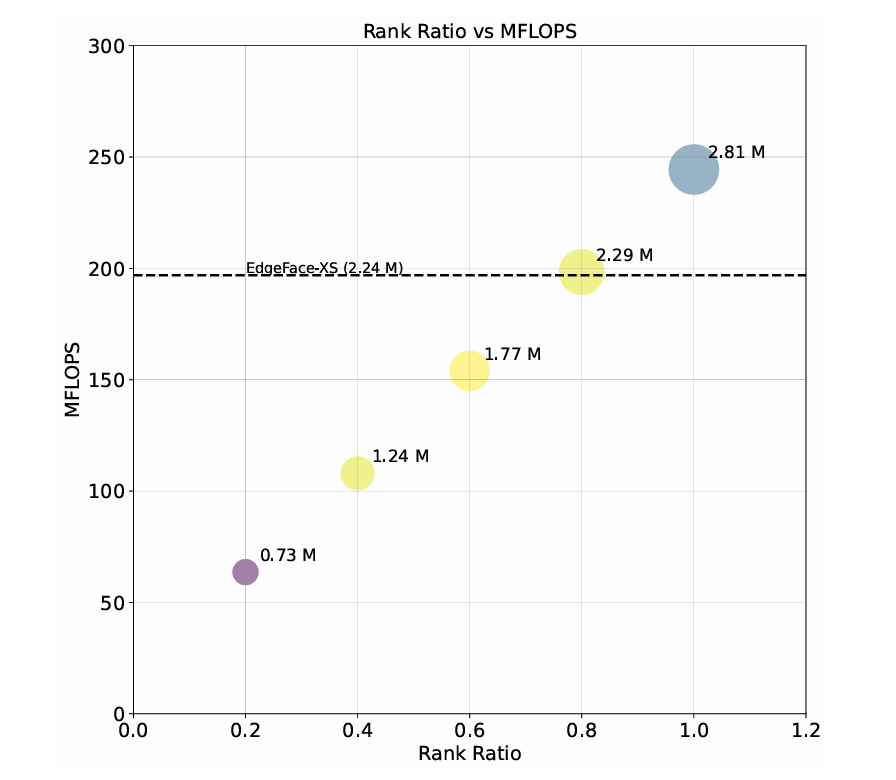
\includegraphics[width=0.65\textwidth]{images/fig3.2.3.png} % đường dẫn 
    \caption{Ảnh hưởng của tham số \textit{Rank-ratio} ($\gamma$) đến số lượng tham số của mô hình (MPARAMS) và số phép nhân-cộng (MFLOPs). 
    Đường nét đứt thể hiện giá trị tham chiếu của mô hình gốc khi sử dụng lớp tuyến tính thông thường. 
    Có thể thấy khi $\gamma$ giảm, số tham số và FLOPs giảm đáng kể, trong khi vẫn duy trì hiệu suất gần như không đổi.}
    \label{fig:lora_lin_rank}
    
\end{figure}

\begin{itemize}
    \item Khi $\gamma < 0.8$, số tham số và FLOPs giảm đáng kể so với lớp tuyến tính chuẩn.
    \item Ở $\gamma \approx 0.6$, EdgeFace đạt \textbf{sự cân bằng tối ưu}: giảm khoảng $20\%$ số tham số và FLOPs, trong khi suy giảm hiệu suất dưới $0.5\%$.
\end{itemize}
Điều này chứng tỏ LoRaLin mang lại khả năng nén mô hình hiệu quả với trade-off tối thiểu về độ chính xác.

\paragraph{Triển khai và minh họa.} 
Trong PyTorch, LoRaLin có thể được triển khai đơn giản bằng cách xâu chuỗi hai lớp tuyến tính:
\begin{itemize}
    \item \texttt{lin1}: ánh xạ từ \texttt{in\_feat} $\to$ \texttt{rank}.
    \item \texttt{lin2}: ánh xạ từ \texttt{rank} $\to$ \texttt{out\_feat}.
\end{itemize}
Nhờ thiết kế này, LoRaLin có thể thay thế trực tiếp các lớp tuyến tính truyền thống trong EdgeFace mà không làm phức tạp thêm quá trình huấn luyện hay suy luận. Trên thực tế, toàn bộ các lớp fully connected trong EdgeFace đều được thay bằng LoRaLin để tối ưu hiệu quả tính toán.

\paragraph{Kết luận.} 
Tóm lại, \textbf{LoRaLin} là một giải pháp gọn nhẹ và hiệu quả để giảm số tham số và FLOPs trong các lớp fully connected. Với cơ chế phân tích hạng thấp và khả năng điều chỉnh linh hoạt qua $\gamma$, LoRaLin cho phép EdgeFace duy trì chất lượng biểu diễn embedding gần như không suy giảm, đồng thời đáp ứng yêu cầu triển khai trên thiết bị biên.

\subsection{Chi tiết huấn luyện}
\subsubsection{Chiến lược huấn luyện}

EdgeFace được huấn luyện nhằm tối ưu hóa hiệu suất nhận diện khuôn mặt trong điều kiện hạn chế tài nguyên trên thiết bị biên. 
Quy trình huấn luyện tận dụng tập dữ liệu quy mô lớn kết hợp với các chiến lược tối ưu hóa để vừa nâng cao độ chính xác, vừa duy trì tính gọn nhẹ của mô hình \cite{george2024edgeface}.

\textbf{Dataset.} Mô hình được huấn luyện trên các tập con WebFace12M và WebFace4M, được trích xuất từ WebFace260M. 
Các ảnh trong tập dữ liệu này đã được căn chỉnh khuôn mặt và chuẩn hóa độ phân giải về $112\times112$, phù hợp với tiêu chuẩn của các hệ thống nhận diện khuôn mặt.

\textbf{Tiền xử lý và tăng cường dữ liệu.} Dữ liệu đầu vào được chuyển đổi thành tensor và chuẩn hóa về khoảng $[-1,1]$. 
Quá trình tăng cường dữ liệu được thực hiện bằng thư viện DALI, bao gồm các phép biến đổi như chuyển đổi ngẫu nhiên sang thang xám, thay đổi kích thước, và làm mờ, nhằm tăng tính đa dạng và tính khái quát của mô hình.

\textbf{Chi tiết huấn luyện.} Mô hình được huấn luyện trên 4--8 GPU Nvidia RTX 3090 (24GB) với chiến lược \textit{distributed training}. 
Optimizer AdamW kết hợp với hàm mất mát CosFace được sử dụng để tối ưu embedding. 
Lịch trình learning rate theo \textit{polynomial decay with restarts} giúp mô hình hội tụ ổn định. 
Batch size dao động từ 256 đến 512 tùy thuộc vào kích thước mô hình, và PartialFC được áp dụng để xử lý số lượng lớn danh tính trong tập dữ liệu.

\textbf{Inference.} Trong giai đoạn suy luận, \textit{classification head} được loại bỏ. 
Mô hình chỉ sử dụng vector embedding 512 chiều làm biểu diễn đặc trưng cho so sánh và truy hồi khuôn mặt.

Tóm lại, quy trình huấn luyện của EdgeFace kết hợp dữ liệu quy mô lớn, tiền xử lý hiệu quả, và các kỹ thuật tối ưu hóa hiện đại, từ đó đạt được hiệu suất cao trong khi vẫn đảm bảo khả năng triển khai trên thiết bị biên.


\chapter{Thực nghiệm}
\label{Chapter 4}

\section {Giới thiệu thực nghiệm}
% Giới thiệu ngắn gọn mục đích thực nghiệm, nhấn mạnh so sánh EdgeFace (Lightweight) với baseline OPQN, tập trung vào tính tinh gọn và khả năng mở rộng. 

% Cần có:
% Mục tiêu: Đánh giá accuracy, MAP, P@10, speed (ms/query), params.
% Các biến thể: Freeze, unfreeze, CosFace, ArchFace
% Dataset: Facescrub seen (chi tiết số ảnh/danh tính), unseen/VGGface2
% So sánh: Với OPQN, nhấn mạnh đóng góp mới

%K Kế hoạch viết: Bắt đầu bằng đoạn tổng quát, thêm lý do chọn dataset (intra-class variances cao).

Trong chương này, chúng tôi trình bày các thực nghiệm nhằm đánh giá hiệu quả của mô hình EdgeFace - một kiến trúc tinh gọn được đề xuất cho nhiệm vụ truy xuất ảnh mặt người trên tập dữ liệu lớn - so với mô hình cơ sở OPQN sử dụng mạng xương sống ResNet20 \cite{opqn}. Các thực nghiệm tập trung vào hai khía cạnh chính: (i) độ chính xác truy xuất, được đo bằng chỉ số trung bình của độ chính xác trung bình (MAP) và Độ chính xác trong T kết quả hàng đầu (P@T), nhằm đánh giá khả năng trả về các kết quả liên quan một cách chính xác; và (ii) tốc độ truy vấn, được đo lường bằng thời gian trung bình mỗi truy vấn(ms/query), nhằm nhấn mạnh tính hiệu quả thực tiễn của mô hình trong môi trường dữ liệu lớn với tài nguyên hạn chế. 

Để đạt được mục tiêu trên, chúng tôi thử nghiệm các biến thể của EdgeFace, bao gồn: Freeze Backbone (giữ cố định các lớp thấp để giảm quá khớp và tăng tốc độ huấn luyện), Unfreeze Backbone (huấn luyện toàn bộ mạng xương sống để học các đặc trưng sâu hơn), huấn luyện lại với CoseFace (xử dụng biên độ cosine để tăng khả năng phân biệt), và huấn luyện lại với ArcFace (sử dụng biên độ góc để cải thiện khả năng tổng quát hoá trên các danh tính chưa từng thấy). Các thực nghiệm hiện tại chủ yếu được thực hiện trên tập dữ liệu FaceScrub với thiết lập các danh tính đã tâhys, nơi tập huấn luyện và kiểm tra chia sẻ cùng các danh tính, nhằm đánh giá hiệu suất cơ bản của mô hình. Các kết quả trên các danh tính chưa thấy (kiểm tra trên các danh tính không có trong huấn luyện) và tập dữ liệu VGGFace2 đang được cập nhật và sẽ được bổ sung theo hướng nghiên cứu trong bài báo gốc \cite{opqn}.

Phần thực nghiệm nhằm chứng minh rằng EdgeFace không chỉ tinh gọn hơn về số lượng tham số (Giảm khoảng 92\% so với ResNet20) mà còn có khả năng duy trì hoặc cải thiện hiệu xuất so với mô hình cơ sở, đặc biệt trong bối cảnh truy xuất ảnh mặt người với các biến thể ngoại lớp lớn (kiểu dáng, ánh   sáng, biểu cảm) và các khoảng cách nội lớp nhỏ. Chúng tôi sẽ phân tích chi tiết từng khía cạnh, bao gồm lý do cho các kết quả bất ngờ (như MAP thấp ở một số biến thể), các đánh đổi giữa độ chính xác và tốc độ, cũng như đề xuất các hướng tối ưu hoá để khắc phục hạn chế. Các kết quả sẽ được trình bày qua bảng biểu và hình ảnh minh hoạ, với phân tích liên hệ chặt chẽ đến mục tiêu đề tài: Phát triển một kiến trúc tinh gọn phù hợp cho truy xuất ảnh mặt người trên tập dữ liệu có khả năng mở rộng.

\section {Thiết lập thực nghiệm}
% Mục tiêu: Cung cấp chi tiết để tái lập, mô tả dataset chuẩn, cách xử lý. Nhấn mạnh môi trường Kaggle (lightweight phù hợp edge), thêm params count để highlight lightweight
Phần này trình bày chi tiết về môi trường thực nghiệm, tập dữ liệc, các chi tiết triển khai và các chỉ số đánh giá được sử dụng để đảm bảo tính tái lập và minh bạch trong quá trình nghiên cứu. Thiết lập được thiết kế để tối ưu hoá hiệu quả của mô hình EdgeFace - một kiến trúc tinh gọn được đề xuất - trong nhiệm vụ truy xuất ảnh mặt người trên tập dữ liệu lớn, đồng thời so sánh với mô hình cơ sở OPQN sử dụng mạng xương sống ResNet20 \cite{opqn}. Các thông số được chọn dựa trên bài báo gốc nhưng được điều chỉnh để phù hợp với đặc điểm tinh gọn của EdgeFace, nhằm nhấn mạnh tính hiệu quả và khả năng triển khai trên các thiết bị có tài nguyên hạn chế. Đặc biệt, chúng tôi sử dụng hai phiên bản kích thước ảnh khác nhau cho tập dữ liệu FaceScrub: 32x32 pixel cho mô hình gốc (OPQN với ResNet20) để đảm bảo tính nhất quán khi so sánh kết quả trong bài báo gốc, và 112x112 pixel cho các biến thể EdgeFace để phù hơp với yêu cầu đầu vào của kiến trúc này \cite{george2024edgeface}, giúp tối ưu hoá hiệu suất huấn luyện và suy diễn.

\subsection{Bộ dữ liệu}
Chúng tôi của dụng tập dữ liệu Facescrub \cite{facescrub} làm nguồn dữ liệu chính trong giai đoạn thực nghiệm ban đầu, do đặc điểm phù hợp với nhiệm vụ truy xuất ảnh mặt người với quy mô vừa phải. Tập dữ liệu này chứa tổng cộng 106,863 ảnh mặt của 530 danh tính của các nhân vật nổi tiếng, với trung bình khoảng 200 ảnh mỗi danh tính, đảm bảo sự đa dạng về kiểu dáng, ánh sáng và biểu cảm - những yếu tố gây ra các biến thể nội lớp lớn, đồng thời tạo ra các khoảng cách ngoại lớp nhỏ giữa các cá nhân có ngoại hình tương đồng. Trong thực nghiệm, tập huấn luyện bao gồm 38,722 ảnh tương ứng với 530 dánh tính, và tập kiểm tra chứa 2,550 ảnh với cùng số lượng danh tính. Số lượng khối dữ liệu và vòng lặp lần lượt là 152 cho huấn luyện và 10 cho kiểm tra, với kích thước khối dữ liệu được đặt là 256 để cân bằng giữa hiệu suất tính toán và sử dụng bộ nhớ trên GPU.

Để đảm bảo tính nhất quán và phù hợp với các mô hình khác nhau, chúng tôi áp dụng hai phiên bản kích thước ảnh cho FaceScrub:
\begin{itemize}
    \item \textbf{Phiên bản 32x32 pixel}: Được sử dụng cho mô hình gốc OPQN với mạng xương sống ResNet20, nhằm tái hiện và so sánh trực tiếp với kết quả trong bài báo gốc \cite{opqn}. Phiên bản này tập trung vào tính tinh gọn và hiệu quả dựa trên dữ liệu kích thước nhỏ.
    \item \textbf{Phiên bản 112x112 pixel}: Được sụng cho các biến thể của EdgeFace, phù hợp với yêu cầu đầu vào của kiến trúc này để tận dụng tối đa các đặc trưng được học từ mô hình được huấn luyện sẵn, giúp cải thiện độ phân biệt mà không làm tăng đáng kể độ phức tạp tính toán.
\end{itemize}

Quy trình tiền xử lý dữ liệu được thực hiện một cách cẩn thận để đảm bảo chất lượng ảnh đầu vào, giảm thiểu nhiễu và tăng cường tính nhất quán. Quy trình này bao gồm các bước sau:

\begin{enumerate}
    \item \textbf{Phát hiện khuôn mặt}: Sử dụng thư viện dlib để phát hiện các khuôn mặt trong ảnh gốc. Chúng tôi chọn khuôn mặt lớn nhất (dựa trên diện tích khung bao quanh ảnh) để tập trung vào đối tượng chính, tránh các khuôn mặt phụ hoặc nhiễu nền.
    \item \textbf{Căn chỉnh với biên}: Giữ nguyên ảnh gốc và thêm biên xung quanh khung bao quanh ảnh để mở rộng vùng khuôn mặt, tránh cắt sát cạnh gây mất thông tin. 
    \item \textbf{Thay đổi kích thước để chống méo hình}: Chúng tôi thực hiện việc thay đổi kích thước theo hai bước, đầu tiên là phóng đại lên kích thước lớn hơn, sau đó thu nhỏ về kích thước mục tiêu. Cụ thể:
    \begin{itemize}
        \item Cho phiên bản 32x32: Phóng to lên 64x64 pixel, sau đó thu nhỏ xuống 32x32 pixel sử dụng phương pháp nội suy tuyến tính để giữ chi tiết mịn màng.
        \item Cho phiên bản 112x112: Phóng to lên 224x224 pixel, sau đó thu nhỏ xuống 112x112 pixel với cùng phương pháp, giúp bảo tồn các đặc trung hình ảnh quan trọng cho EdgeFace.
    \end{itemize}
\end{enumerate}

Thực nghiệm được tiến hành trong hai thiết lập chính:
\begin{itemize}
    \item \textbf{Seen identities}: Tập huấn luyện và kiểm tra sử dụng cùng các danh tính nhằm đánh giá hiệu suất cơ bản khi mô hình đã được huấn luyện trên dữ liệu quen thuộc. Thiết lập này tuân theo giao thức trong \cite {opqn}, tập trung vào các chỉ số MAP và P@K (K từ 10 đến 100, bước 10) để so sánh với các phương pháp tiên tiến.
    \item \textbf{Unseen identities}: Tập kiểm tra chứa các danh tính không xuất hiện trong tập huấn luyện, được mô phỏng bằng cờ \texttt{--cross-dataset} trong code để phản ánh tính kịch bản thực tế nơi số lượng các danh tính mới tăng dần. Thiết lập này quan trọng để đánh giá khả năng tổng quát hoá và khả năng mở rộng của mô hình, nhưng hiện đagn dượdc cập nhât do yêu cầu tài nguyên tính toán cao hơn.
\end {itemize}

Bên cạnh đó, chúng tôi dự kiến mở rộng sang tập dữ liệu VGGFace2 trong tương lai để kiểm tra tính mở rộng trên dữ liệu quy mô lớn. Tập dữ liệ này bao gồm 3,31 triệu ảnh của 9,131 các danh tính, với phân chia chính thức: 8,631 các danh tính cho huấn luyện và 500 danh tính cho kiểm tra. Theo giao thức trong OPQN, 50 ảnh mỗi danh tính sẽ được sử dụng cho tập kiểm tra, phần còn lại cho cơ sở dữ liệu truy xuất. Các ảnh trong FaceScrub đã được xử lý trước bằng cách cắt và thay đổi kích thước về kích thước 32x32 pixel, trong khi VGGFace2 sẽ được căn chỉnh bằng MTCNN và thay đổi kích thước về 112x112 pixel để đảm bảo tính nhất quán.

\subsection{Cài đặt chi tiết}
Thực nghiệ được triển khai trên nền tảng Kaggle với hai GPU NVIDIA T4 (Mỗi GPU 16GB VRAM), hệ điều hành Linux, và framework PyTorch phiên bản 1.9 để tận dụng tính linh hoạt trong phát triển mô hình học sâu. Mô hình EdgeFace được sử dụng làm mạng sương sống thay thế cho ResNet20 trong OPQN, với mục tiêu giảm độ phức tạp tính toán và số lượng tham số trong khi vẫn duy trì hiệu suất. EdgeFace là một kiến thức gọn nhẹ được thiết kế đặc biệt cho các thiết bị biên, với tổng số tham số có thể huấn luyện khoảng 1,771,516 (~1.8 triệu), giảm đáng kể so với 24,562,496 (~24 triệu) tham số của ResNet20 - tương ứng với mức giảm 92\%, giúp tối ưu hoá hiệu suất trên các hệ thống có tài nguyên hạn chế. Việc sử dụng kích thước đầu vào 112x112 cho EdgeFace (so với 32x32 cho ResNet20) đảm bảo mô hình khai thác tối đa các đặc trung chi tiết từ ảnh, phù hợp với yêu cầu thiết kế của EdgeFace mà không làm tăng quá mức độ phức tạp.

Chúng tôi thử nghiệm bốn biến thể chính của EdgeFace để khám phá các đánh đổi giữa độ chính xác và tốc độ.

\begin{itemize}
    \item \textbf{Freeze backbone}: Giữ cố định các layer conv1 và layer1 (chứa các đặc trưng cấp thấp từ quá trình tiền huấn luyện), chỉ huấn luyện các layer cao hơn. Phương pháp này nhằm giảm nguy cơ quá khớp trên tập dữ liệu nhỏ và tăng tốc độ huấn luyện bằng cách hạn chế số lượng tham số được cập nhật.
    \item \textbf{Unfree backbone}: Huấn luyện toàn bộ mạng xương sống từ đầu hoặc tinh chỉnh để tận dung khả năg học các đặc trưng sâu hơn. Phương pháp này có tiềm năng cải thiện độ phân biệt nhưng đễ dẫn đến hiện tượng quá khớp nếu không có đủ dữ liệu hoặc chuẩn hoá không đủ.
    \item \textbf{Khởi tạo trọng số, tiền huấn luyện với CosFace}: Chúng tôi khởi tạo các trọng số của mạng xương sống EdgeFace băgnf cách tiền huấn luyện với hàm mất mát CosFace (tham số co giãn $s = 30$, biên độ $m = 0.2$). Kỹ thuật này được sử dụng để tối đa hoá độ chặt chẽ nội lớp và khoảng cách ngoại lớp trong không gian đặc trưng nhúng, cung cấp một nền tảng vức chắc cho quá trình huấn luyện lượng tử hoá tiếp theo.
    \item \textbf{Khởi tạo trọng số, tiền huấn luyện với ArcFace}: Chúng tôi khởi tạo các trọng số của mạng xương sống EdgeFace (tham số co giãn $s = 30$, biên độ $m = 0.5$). Kỹ thuật này sử dụng biên độ góc để tăng cường sự phân tách góc giữa các danh tính trong không gian đặc trưng nhúng, tạo ra các đặc trung phân biệt mạnh mẽ hơn. Điều này đặc biệt hữu ích khi mục tiêu là đạt hiệu suất tốt trên các danh tính chưa thấy hoặc trong các kịch bản đánh giá chéo tập dữ liệu. Biến thể này đang được cập nhật.
\end{itemize}

Các tham số chung cho tất cả các biến thể bao gồm: độ dài mã hoá được khảo sát trong khoảng rộng từ 16 đến 48 bit (với các cấu hình cụ thể là 16, 24, 36, 48 bit). Cụ thể, cấu hình 48 bit được đạt được với số lượng bộ mã $num=8$ và số lượng từ mã mỗi bộ mã $words=64$ (do $8 \times \log_2(64) = 48$). Chiều đặc trưng nhúng đầu ra được đặt là 512 để cân bằng giữa khả năng biểu diễn và hiệu quả sử dụng bộ nhớ. Kích thước khối dữ liệu được thiết lập là 256 để phù hợp với giới hạn VRAM của GPU T4x2 mà không gây lỗi hết bộ nhớ (OOM). Quy trình huấn luyện được chia thành hai giai đoạn:
\begin{itemize}
    \item \textbf{Giai đoạn tiền huấn luyện}: Sử dụng thuật toán tối ưu hoá AdamW với hai mức độ học tập khác nhau: 0.0001 cho phần mạng xương sống và 0.001 cho phần đầu metric. Chúng tôi áp dụng bộ điều chỉnh tốc độ học CosineAnnealingLR để điều chỉnh tốc độ học một cách mượt mà theo hàm cosine, cho phép mô hình giảm tốc độ học dần về 0 khi kết thúc quá trình huấn luyện. Quá trình này được chạy trong 50 vòng lặp. Các kỹ thuật tăng cường dữ liệu được áp dụng để tăng cường khả năng tổng quát hoá trước các biến thiên trong dữ liệu bao gồm: Cắt ảnh ngẫu nhiên và lật ảnh ngẫu nhiên. 
    \item \textbf{Giai đoạn tinh chỉnh OrthoPQ}: Chúng tôi sử dụng thuật toán tối ưu hoá SGD (Stochastic Gradient Descent) với tốc độ học tập ban đầu là 0.1. Các siêu tham số chính được thiết lập dữ trên nghiên cứu OPQN gốc, bao gồm: Biên độ $m = 0.4$, trọng số dư thừa $miu = 0.1$, hệ số co giãn $sc = 30$. Chúng tôi cũng áp dụng bộ điều chỉnh tốc độ học ReduceLROnPlateau để điều chỉnh tốc độ học dựa trên giá trị hàm mất mát trên tập huấn luyện, giảm tốc độ học khi mô hình không có sự cải thiện. Giai đoạn này được chạy trong 300 vòng lặp để tối ưu hoá hiệu suất lượng tử hoá và hiệu suất truy vấn. 
\end{itemize}

Toàn bộ mã nguồn được phát triển dựa trên quá trình triển khai OPQN nhưng được điều chỉnh để tích hợp mạng xương sống EdgeFace và được xử lý các phiên bản kích thước ảnh khác nhau. Thời gian huấn luyện trung bình dao động từ 5 đến 10 giờ cho mỗi biến thể trên Kaggle, tuỳ thuộc vào độ dài mã hoá. 

\subsection{Evaluation Metric}
Để đánh giá hiệu quả toàn diện của mô hình, chúng tôi sử dụng ba chỉ số chính, phù hợp với các nghiên cứu trong lĩnh vực truy xuất ảnh mặt người:
\begin{itemize}
    \item \textbf{Độ chính xác trung bình - MAP}: MAP là chỉ số đo lường độ chính xác trung bình trên toàn bộ các truy vấn, được tính dựa trên đường cong Precision-Recall. Chỉ số này phản ánh khả năng trả về các mục tiêu liên quan (cùng danh tính) ở các vị trí cao (top ranks) và là một thước đo quan trọng cho hiệu suất truy xuất ở quy mô lớn.
    \item \textbf{Độ chính xác tại Top-K - P@K}: P@K thể hiện tỷ lệ ảnh đúng (cùng danh tính) trong $K$ kết quả đầu tiên được trả về, với K được khảo sát trong phạm vi từ 10 đến 100 với bước nhảy 10, theo giao thức trong bài báo gốc. Chỉ số này phản ánh hiệu suất thực tế của hệ thống đối với người dùng, vì họ thường chỉ xem xét các kết quả hàng đầu.
    \item \textbf{Tốc độ truy vấn - ms/query}: Chỉ số này là thời gian trung bình cần thiết để thực hiện mỗi truy vấn. Nó được tính bằng tổng thời gian thực thi hàm tính khoảng cách bất đối xứng trong OPQN (PqDisRet\_Ortho) chia cho tổng số lượng ảnh kiểm tra (khoảng 2,550 ảnh trong FaceScrub). Việc báo cáo tốc độ truy vấn là một đóng góp mới của nghiên cứu nhằm nhấn mạnh tính hiệu quả của mô hình trên các thiết bị nhẹ, do bài báo gốc không công bố chỉ số này.
\end{itemize}

Các chỉ số được báo cáo riêng biệt cho các danh tính được thấy và chưa thấy (unseen và P@K đang được cập nhật). Ngoài ra chúng tôi đo lường số lượng tham số có thể huấn luyện để đinh lượng mức độ tinh gọn của kiến trúc. Nếu cần thiết, các phân tích thống kê như kiểm định t-test sẽ được xem xét để xác định mức độ ý nghĩa thống kê của các cải thiện trong MAP, nhưng hiện tại, chúng tôi ưu tiên phân tích mô tả để làm rõ các xu hướng chính.

\section {Kết quả và phân tích}

\section {Nghiên cứu cắt bỏ}

% Công trình của tác giả (nếu không có thì comment 02 dòng dưới)
\addcontentsline{toc}{chapter}{Danh mục công trình của tác giả}
\chapter*{Danh mục công trình của tác giả}
\label{Appendix1}

\begin{enumerate}
\item Tạp chí ABC
\item Tạp chí XYZ
\end{enumerate}

% In tài liệu tham khảo
\addcontentsline{toc}{chapter}{Tài liệu tham khảo}
\printbibheading[title={Tài liệu tham khảo}]



%\printbibliography

\printbibliography[heading=subbibliography, title={Tiếng Việt}, keyword=Viet, resetnumbers=true]

\DeclareNameAlias{sortname}{last-first}
\DeclareNameAlias{default}{last-first}

\printbibliography[heading=subbibliography, title={Tiếng Anh}, notkeyword=Viet, resetnumbers=4] 
% ===================================================================== %
% CHÚ Ý: phải gán lại resetnumbers=số tài liệu tham khảo tiếng Việt + 1 %
% ===================================================================== %

% Phần phụ lục
\appendix

\chapter{Ngữ pháp tiếng Việt}
\label{Appendix1}

Đây là phụ lục.
\chapter{Ngữ pháp tiếng Nôm}
\label{Appendix2}

Đây là phụ lục 2.

\end{document} 